\documentclass[a4paper,fleqn]{cas-sc}

% ===== Packages =====
\usepackage[numbers,sort&compress]{natbib}
\usepackage{amsmath,amsfonts,amssymb}
\usepackage{booktabs}
\usepackage{enumitem}
\usepackage{subcaption}
\usepackage{float}
\usepackage{multirow}
\usepackage{array}
\usepackage{tabularx}
\usepackage{bm}
\usepackage{siunitx}
\usepackage{algorithm}
\usepackage{algpseudocode}
\usepackage{graphicx}
\usepackage{xcolor}
\usepackage{hyperref}
\hypersetup{colorlinks=true, linkcolor=blue, citecolor=blue, urlcolor=blue}
\usepackage{lineno}
\linenumbers

% ===== Custom Commands =====
\newcommand{\Mzero}{M_0}
\newcommand{\Mphys}{M_\text{phys}}
\newcommand{\Mtl}{M_\text{TL}}
\newcommand{\Mtlphys}{M_\text{TL+phys}}
\newcommand{\Mrand}{M_\text{rand}}
\newcommand{\MAE}{\text{MAE}}
\newcommand{\eg}{\textit{e.g.}}
\newcommand{\ie}{\textit{i.e.}}

\begin{document}

\let\WriteBookmarks\relax
\def\floatpagepagefraction{1}
\def\textpagefraction{.001}

\shorttitle{PBTL for MIM Absorber Surrogates}
\shortauthors{S.-B.~Choi, J.~Kim, C.-M.~Kang}

\title[mode=title]{Physics-Based Transfer Learning for Neural Network Surrogates of Metal--Insulator--Metal Absorbers}

\author[1]{Sang-Bae Choi}
\cormark[2]
\fnmark[1]
\ead{sbchoi129@gmail.com}

\author[2,3]{Joonhyub Kim}
\ead{kim4539@pusan.ac.kr}

\author[2,3]{Chang-Mo Kang}
\cormark[1]
\ead{fd1kcm@pusan.ac.kr}

\affiliation[1]{organization={Independent Researcher},
                city={Busan},
                postcode={46264},
                country={Republic of Korea}}
\affiliation[2]{organization={Department of Nanomechatronics Engineering, Pusan National University},
                city={Busan},
                postcode={46241},
                country={Republic of Korea}}
\affiliation[3]{organization={School of Transdisciplinary Engineering, Pusan National University},
                city={Busan},
                postcode={46241},
                country={Republic of Korea}}

\cortext[cor1]{Corresponding author}
\cortext[cor2]{Co-corresponding author}
\fntext[fn1]{Independent researcher; this work was carried out independently, without institutional affiliation, and correspondence with this author is therefore via the personal email address listed.}

\begin{abstract}
Cross-fidelity transfer learning is widely used to accelerate neural-network (NN) surrogate modeling of nanophotonic structures, but published reports show inconsistent outcomes: the same protocol yields large gains for some structures and negligible or even negative gains for others, with no published raw-output criterion for telling them apart in advance. We close this gap with the following results for physics-based transfer learning (PBTL) of metal--insulator--metal (MIM) absorber surrogates. (i)~We decompose the conventional PBTL protocol into its two components---analytical physics features and transfer-matrix-method (TMM)-pre-trained weight initialization---and quantify each separately on three structurally distinct Cr-based MIM absorbers (Cr/SiO$_2$, with an added TiO$_2$ spacer in Structure~A): physics features yield a robust $4$--$30\%$ mean absolute error (MAE) reduction across all three Cr structures, while weight-level transfer ($\Mtl$ vs.\ $\Mzero$) is positive for every structure and training-set size but strongly \emph{fidelity-graded}: at a matched $n=350$ the cross-structure benefit tracks TMM--rigorous coupled-wave analysis (RCWA) spectral fidelity ($+31.3\%$ for A, $+13.5\%$ for B, $+9.7\%$ for C), and peaks at $+49.7\%$ for Structure~A at the smallest pool ($n=50$). A corrected Au/SiO$_2$ cross-material check confirms positive weight-level transfer for both Structures~A and~B---stronger for A (up to $+38\%$) and weaker but still positive for B (up to $+28\%$, decaying toward the saturated pool). Au-A and Au-B have near-identical TMM--RCWA fidelity, so we do not attribute the A-vs-B Au gap to fidelity grading (Sections~\ref{sec:material_generalization}, Supplementary S9). (ii)~We introduce a simple, raw-output indicator that correlates with this variability: a joint pilot-set diagnostic combining the TMM--RCWA spectral Pearson correlation $r$ (shape component) and absolute MAE (amplitude component) in the target operating band. Controlled noise injection on Structure~A drives a monotone decrease of the weight-transfer benefit as source fidelity degrades---from $+47\%$ at full fidelity to $-58\%$ at zero fidelity (Spearman $\rho=-1.0$); consistent with the cross-structure result, the operating-band absolute MAE predicts this benefit markedly better than the shape correlation~$r$ ($|$Pearson$|=0.98$ vs.\ $0.81$). Across the three real structures the amplitude component (MAE) orders the benefit monotonically while shape correlation alone does not, so both components must be considered jointly (Sections~\ref{sec:cross_structure}, \ref{sec:guidelines}). Unlike previously proposed transferability metrics, the indicator requires neither PCA projection nor a pre-trained model. (iii)~Genuine negative transfer was not observed for any of the three structures at its native fidelity; it arises only under \emph{controlled} source degradation---near zero for the high-fidelity Structure~A, but already at moderate noise ($\sigma=0.10$) for the lower-fidelity Structures~B and~C---so reliable pre-screening is best served by the \emph{joint} $r$-and-MAE diagnostic, with the amplitude (MAE) component---not shape correlation alone---ordering the benefit. Operationally, a pilot set of $50$ RCWA samples (${\sim}15$--$30$\,min on a single GPU) suffices to estimate both components within the target band before committing to the full RCWA-data-generation and training pipeline (${\sim}4$--$5$\,h); a bootstrap analysis confirms both components (shape $r$ and amplitude MAE) are stable at $n_\text{pilot}\leq 50$ on the corrected data, reliably flagging low-fidelity transfer sources. The diagnostic framework is solver-pair-agnostic and may extend to other cheap--expensive simulator combinations in computational photonics, pending validation outside the MIM-absorber family tested here.
\end{abstract}

\begin{keywords}
metasurface \sep metamaterial absorber \sep machine-learning-driven design \sep physics-based transfer learning \sep neural-network surrogate \sep multi-fidelity modeling \sep rigorous coupled-wave analysis
\end{keywords}

\maketitle

% =====================================================================
% 1. INTRODUCTION
% =====================================================================
\section{Introduction}
\label{sec:intro}

Metal--insulator--metal (MIM) metamaterial absorbers are a workhorse class of sub-wavelength photonic nanostructures that enable wavelength-selective, near-perfect absorption from the visible to near-infrared spectrum~\cite{landy2008perfect}. Their applications range from thermal emitters and photodetectors to structural color filters and radiative cooling. Optimizing these structures requires exploring high-dimensional design spaces---combinations of period, feature sizes, layer thicknesses, and incidence angles---that govern complex electromagnetic interactions including Fabry--P\'{e}rot cavity resonance, plasmonic coupling, and Fano interference. The same design challenges arise across the broader family of resonant metasurfaces, plasmonic nanostructures, and photonic-crystal absorbers, motivating methodologies that generalize across geometries.

Full-wave numerical methods such as rigorous coupled-wave analysis (RCWA) provide accurate spectral predictions but are computationally expensive: a single MIM simulation with oblique incidence and fine spatial discretization typically takes tens of seconds to minutes on a GPU (in our setup, $17$--$33$\,s per $100$-wavelength spectrum on an RTX~4070 Ti SUPER), so generating the thousands of samples needed for high-dimensional design-space exploration costs many hours to days. Neural network surrogates offer a path to real-time spectral prediction, but training them typically requires thousands of RCWA simulations~\cite{so2020deep,liu2018training}.

The transfer matrix method (TMM) provides analytical solutions for planar multilayer stacks in milliseconds. While TMM cannot capture diffraction from sub-wavelength patterning, it encodes essential thin-film physics: interference, absorption in lossy metals, and energy conservation ($A+R+T=1$). This \emph{approximate but physically meaningful} knowledge can potentially serve as a cheap pre-training signal for neural network surrogates---but it is unclear whether such approximate pre-training helps, and if so, under what conditions. This raises the central question of our study: \textbf{when does pre-training on cheap TMM simulations improve neural network surrogates for complex MIM absorbers, and what is associated with the magnitude of this transfer benefit?}

\subsection{Related Work}

Transfer learning has been widely adopted in computer vision and natural language processing~\cite{pan2010survey,zhuang2021comprehensive}, where pre-training on large corpora and fine-tuning on downstream tasks yields significant data-efficiency gains. In computational photonics, surrogate models based on fully connected networks~\cite{so2020deep}, convolutional architectures~\cite{liu2018training,malkiel2018plasmonic}, physics-informed neural networks~\cite{raissi2019physics}, and neural-operator surrogates~\cite{lu2021deeponet} have shown promise for accelerating electromagnetic simulations~\cite{ma2021deep,jiang2021deep}; recent reviews highlight the growing role of deep learning in photonic structure design~\cite{wiecha2021deep,khatib2022deep,an2019deep,wiecha2024newcomer}. In particular, several recent studies use neural-network surrogates to design metamaterial and metasurface absorbers---for example, the residual fully-connected network of Wang~et~al.~\cite{wang2023innovative} for broadband (visible--near-infrared) perfect absorbers and the deep-learning-based inverse design of mid-wave-infrared metasurface absorbers by Shen~et~al.~\cite{shen2025design}---confirming that NN-driven absorber design is an active research direction. These works concentrate on \emph{achieving} a target device performance via deep learning, however, rather than asking \emph{when} a cheap-to-expensive transfer is beneficial in the first place. Most approaches train surrogates from scratch on full-wave simulation data alone, without leveraging cheaper physics models as pre-training sources. Physics-informed features~\cite{chen2019smart} and multi-fidelity modeling~\cite{peherstorfer2018survey,kennedy2000predicting,fernandez2016review,forrester2007multi} have been explored to improve data efficiency, but a critical gap remains: no systematic study has characterized \emph{when} cross-fidelity transfer learning helps, \emph{when} it fails, and \emph{what measurable physical quantity} is associated with the transition between these regimes.

Four recent studies are most closely related. Qu~et~al.~\cite{qu2019migrating} migrated knowledge between multilayer-film tasks within one solver ($50.5\%$ best-case error reduction) and noted same-solver negative transfer in some settings, but did not address cross-fidelity transfer or a pre-screening diagnostic. Cheng~et~al.~\cite{chen2024tl_mdn} performed sequential transfer between mixture density networks of increasing complexity, all drawn from one high-fidelity COMSOL solver. Kim and Kim~\cite{kim2025pbtl}, who independently coined ``physics-based transfer learning'' (PBTL), reported ${\sim}50\%$ training-data reduction for quantum-cascade-laser design by transferring active-region weights into the full-device model---again one simulator at both stages. Most comparably, Peng~et~al.~\cite{peng2024nanophotonics} pre-trained a ResNet across metamaterial geometries and polarizations within a single discrete-dipole-approximation (DDA) tier and proposed a PCA-projected far-field centroid distance as a transferability indicator, finding transfer \emph{never detrimental}. A detailed head-to-head comparison is deferred to Section~\ref{sec:related_comparison}.

Each stays within a single fidelity tier---transferring between tasks, sub-problems, or architectural variants, but not between distinct simulators with different governing approximations. None characterizes \emph{cross-fidelity} negative transfer or proposes a diagnostic for it, decomposes the gain from physics features versus pre-trained weights, or maps how the benefit is graded by source--target fidelity. Classical multi-fidelity modeling does parameterize the low-to-high-fidelity relationship by a correlation/scaling term (the autoregressive $\rho$ of Kennedy and O'Hagan~\cite{kennedy2000predicting}), establishing that fusion benefit scales with inter-fidelity correlation, and a concurrent physical-transfer-learning network for absorbers (PTLOR-Net~\cite{zhu2025ptlor}) achieves data-efficient cross-band spectrum prediction; both, however, supply a transfer \emph{method}. Our contribution is to \emph{decompose} the source--target agreement into a shape (correlation) and an amplitude (operating-band MAE) component on \emph{raw} simulator outputs---a distinction the single scalar $\rho$ conflates---and to show the amplitude component is the one that orders the transfer benefit. The critical practitioner question---when is a cheap simulator close enough to an expensive one for cross-fidelity transfer to be worth the cost?---thus remains open.

The present work addresses this gap by operating at \emph{true cross-fidelity}---mapping an effective-medium-approximation (EMA) based TMM to full RCWA---where transfer is far from guaranteed, and making four contributions: a raw-output transferability diagnostic, an explicit decomposition of the PBTL protocol, a fidelity-graded transfer gradient with a controlled negative-transfer demonstration, and an operational pre-screening procedure. We detail these next.

\subsection{Contributions}

This work makes four contributions to physics-based transfer learning for photonic surrogates. \emph{First}, we introduce a \textbf{joint pilot-set $r$-and-MAE diagnostic} as a simple, raw-output transferability indicator. The general-ML transferability metrics LEEP~\cite{nguyen2020leep} and LogME~\cite{you2021logme} predict downstream classification accuracy from a \emph{pre-trained model's} embeddings, and in photonics Peng~et~al.~\cite{peng2024nanophotonics} proposed a PCA-projected far-field centroid distance for the same purpose within a single fidelity tier; by contrast, we use the agreement between two \emph{simulator outputs}---the joint Pearson correlation $r$ (shape component) and absolute MAE (amplitude component) between TMM and RCWA spectra on a small pilot set in the target operating band, with no PCA or pre-trained model required---and show that this agreement is associated with the weight-level transfer benefit. The two components are required jointly, since shape correlation alone is insufficient when operating-band amplitude error is high (Section~\ref{sec:tmm_accuracy}, Table~\ref{tab:tmm_fidelity}).

\emph{Second}, we provide an \textbf{explicit decomposition of physics-based transfer learning into two separately quantified components}. Whereas prior PBTL work~\cite{chen2024tl_mdn,kim2025pbtl,peng2024nanophotonics} reports the \emph{combined} effect of physics features and pre-trained weight initialization as a single bundled gain, we disentangle the two components on the same task and the same architecture: physics features deliver a robust $4$--$30\%$ MAE reduction across all three Cr/SiO$_2$ structures (the Au/SiO$_2$ checks are structure-dependent---a sizeable ${\sim}13$--$27\%$ reduction on Structure~A but no consistent standalone gain on Structure~B, where the EMA poorly captures the ring--disk coupling; Supplementary~S9), whereas weight-level transfer ($\Mtl$ vs.\ $\Mzero$) is positive but fidelity-graded, at a matched $n=350$ ordered by fidelity across structures ($+31.3\%$ for A, $+13.5\%$ for B, $+9.7\%$ for C) and peaking at $+49.7\%$ for Structure~A at the smallest pool ($n=50$)---a distinction with direct practical consequences for which component to deploy on a new structure.

\emph{Third}, we establish a \textbf{fidelity-graded transfer gradient together with a controlled demonstration of negative transfer}. Whereas prior cross-fidelity-TL papers in photonics report successes or aggregate failure rates without analyzing what is associated with the magnitude of weight-level transfer (e.g., Peng~et~al.~\cite{peng2024nanophotonics} found transfer ``never detrimental''), we show that across three structurally distinct absorbers the weight-transfer benefit is positive but monotonically graded by operating-band TMM--RCWA fidelity (largest for Structure~A, smallest for Structure~C), with the ordering tracking absolute MAE rather than shape correlation $r$ alone; we then define negative transfer quantitatively ($\mathrm{MAE}(M_\text{TL}) > \mathrm{MAE}(M_0)$) and demonstrate it directly by controlled source-fidelity degradation, which drives the benefit from $+47\%$ down to $-58\%$ as the TMM source is corrupted toward zero fidelity (Section~\ref{sec:tmm_accuracy}).

\emph{Fourth}, we specify an \textbf{operational pre-screening procedure with a concrete sample budget}. Against the qualitative guidance typical of cross-fidelity TL, we define an end-to-end procedure in which a small pilot RCWA run (${\sim}50$ geometries on a single GPU) estimates both diagnostic components in the target operating band and applies the joint heuristic of Section~\ref{sec:guidelines} before committing to the full pre-training pipeline, while controlled noise-injection, a random baseline, and four multi-fidelity baselines (Section~\ref{sec:robustness_summary}) rule out confounders; the resulting guide is calibrated on the structures tested and presented as a conservative working heuristic for the MIM-absorber family, not a universal cutoff.

The remainder of this paper is structured as follows. Section~\ref{sec:methods} describes the three MIM absorber structures, simulation methods, neural network architecture, physics features, and the PBTL framework. Section~\ref{sec:results} presents the 4-way model comparison, mechanistic validation experiments, and robustness ablations. Section~\ref{sec:discussion} synthesizes the findings into practical guidelines and discusses limitations. Section~\ref{sec:conclusion} concludes.

% =====================================================================
% 2. METHODS
% =====================================================================
\section{Methods}
\label{sec:methods}

\subsection{MIM Absorber Structures}
\label{sec:structures}

We study three MIM absorber structures that span distinct electromagnetic regimes (Figure~\ref{fig:structures}), all sharing a 100\,nm Cr ground mirror on a glass substrate.

\subsubsection{Structure A: Asymmetric Dual-Dielectric Dual-Cavity}

The most complex structure features two dielectric spacer layers (SiO$_2$ and TiO$_2$) sandwiched between three patterned/uniform Cr layers. Patterned layers (marked EMA below) are homogenized via the EMA (Eq.~\ref{eq:ema}) when evaluated by TMM. The layer stack from top to bottom is:

\begin{equation}
\text{Air} \mid \underbrace{\text{Cr rect}(t_1)}_{\text{EMA}} \mid \text{SiO}_2(d_1) \mid \text{Cr}(t_\text{mid}) \mid \text{TiO}_2(d_2) \mid \underbrace{\text{Cr sq}(t_2)}_{\text{EMA}} \mid \text{Cr mirror}(100\,\text{nm}) \mid \text{Glass}
\end{equation}

This structure has \textbf{10 design parameters}: period $P \in [300, 600]$\,nm, rectangular patch dimensions $W_x, W_y \in [50, 540]$\,nm, square patch width $W_2 \in [50, 540]$\,nm, metal thicknesses $t_1, t_2 \in [10, 80]$\,nm and $t_\text{mid} \in [5, 30]$\,nm, dielectric spacer thicknesses $d_1, d_2 \in [30, 200]$\,nm, and polar incidence angle $\theta \in [0^\circ, 45^\circ]$.

\subsubsection{Structure B: Ring-Disk Fano Resonance}

A concentric ring-and-disk Cr pattern atop a single SiO$_2$ spacer and Cr mirror. The ring and disk support distinct plasmonic modes that hybridize into Fano resonances. This structure has \textbf{8 design parameters}: $P$, outer ring radius $R_\text{out}$, inner ring radius $R_\text{in}$, disk radius $R_\text{disk}$, Cr thickness $t_\text{Cr}$, SiO$_2$ spacer $d_{\text{SiO}_2}$, polar angle $\theta$, and azimuthal angle $\phi$.

\subsubsection{Structure C: Dual-Polarization Rectangular}

A rectangular Cr patch on SiO$_2$/Cr mirror supporting polarization-dependent absorption along its two principal ($x$/$y$) axes (denoted transverse-electric/transverse-magnetic, TE/TM; these coincide with conventional s/p polarization at normal incidence, and only a small fixed azimuthal angle is applied at oblique incidence). This structure has \textbf{7 design parameters}: $P$, $W_x$, $W_y$, $t_\text{Cr}$, $d_{\text{SiO}_2}$, $\theta$, and $\phi$. The output spectrum has two channels (TE and TM absorptance).

\begin{figure}[htbp]\centering
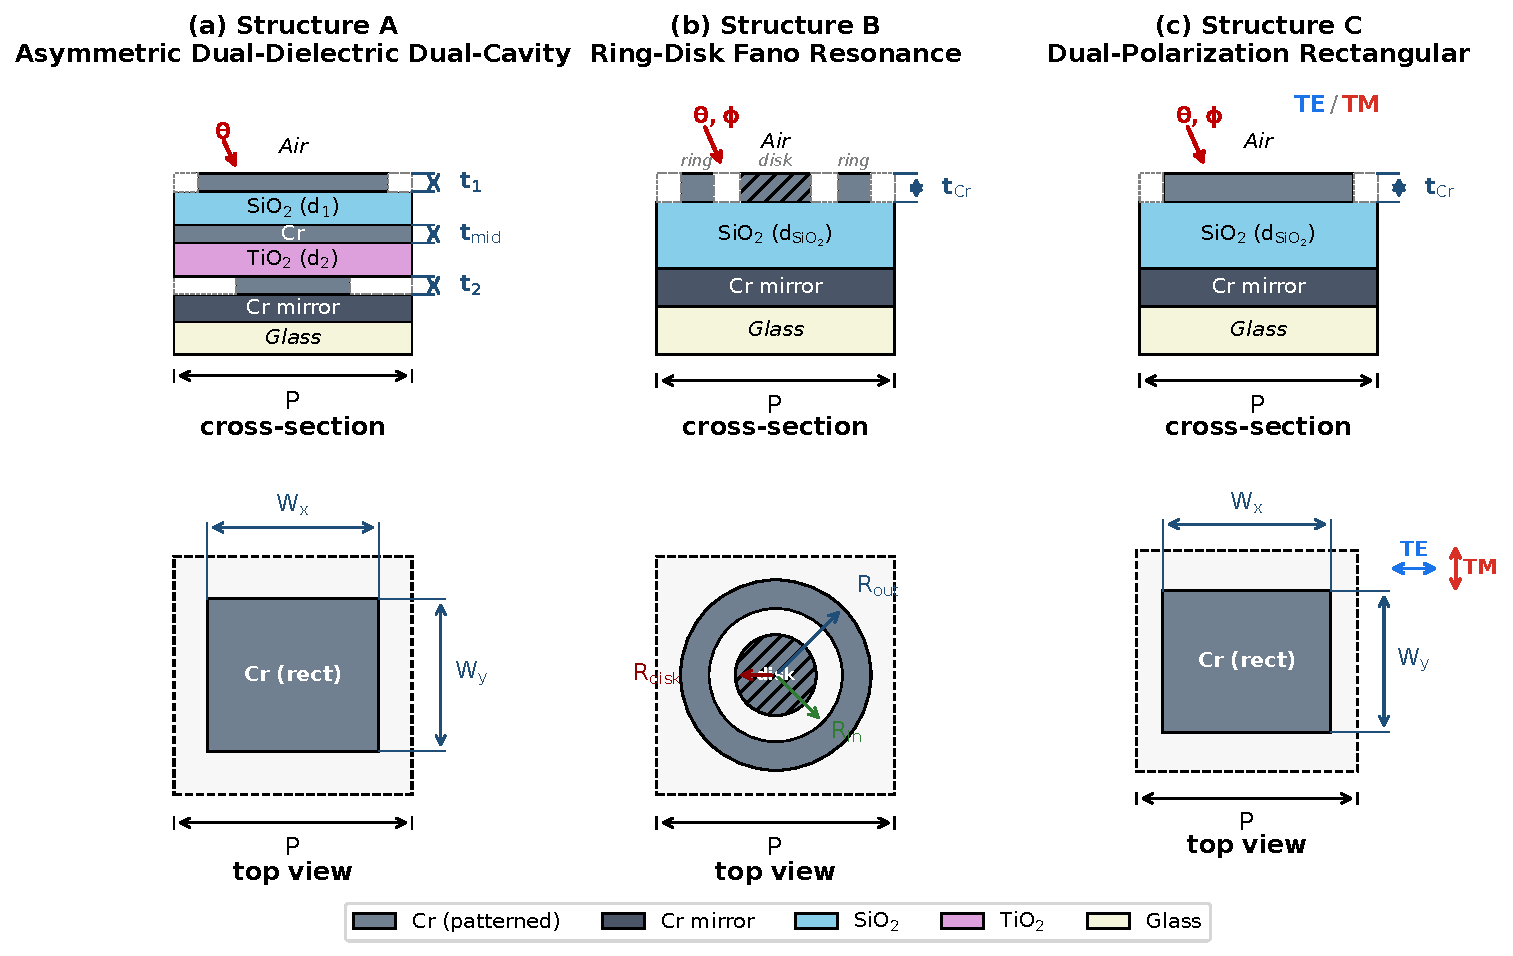
\includegraphics[width=0.985\textwidth]{figures/Figure_1.pdf}
\caption{Schematic illustrations of the three MIM absorber structures studied. Each column shows one structure with its cross-sectional layer stack (top) and the unit-cell top view (bottom) with geometric design parameters. (a)~Structure~A has an asymmetric dual-cavity with two dielectric spacers (SiO$_2$, TiO$_2$) and three Cr layers (10 parameters); the top view shows only the upper rectangular Cr patch ($W_x$, $W_y$), while the buried square Cr patch ($W_2$, in the $t_2$ layer) is omitted for clarity. (b)~Structure~B features a concentric ring-and-disk Cr pattern supporting Fano resonances (8 parameters). (c)~Structure~C uses a single rectangular Cr patch with dual-polarization (TE/TM) output (7 parameters). All structures share a 100\,nm Cr ground mirror on glass.}
\label{fig:structures}
\end{figure}

\subsection{Electromagnetic Simulation Methods}

\subsubsection{Rigorous Coupled-Wave Analysis (RCWA)}
\label{sec:rcwa_methods}

RCWA simulations serve as ground truth. We use the GPU-accelerated \texttt{torcwa} library with a $64 \times 64$ spatial grid and a per-wavelength adaptive Fourier order (raised from a base $N=5$ up to $N=17$ where feature size and anisotropy require it; see the convergence note below). The absorptance spectrum $A(\lambda)$ is computed at 100 wavelengths over the unified $400$--$1800$\,nm operating band ($\Delta\lambda \approx 14.14$\,nm) shared by all three structures (broadband visible-to-NIR absorbers). The native operating-band setting is used for all PBTL training and evaluation; cross-structure fidelity diagnostics in Section~\ref{sec:cross_structure} also report a visible ($400$--$780$\,nm) sub-band breakdown (over the corrected $500$-geometry evaluated pools) for B and C so that the visible-band fidelity of all three structures can be compared on a common grid.

\textbf{Optical constants.} The metal and TiO$_2$ layers use measured tabulated $n,k$ data, while the SiO$_2$ spacer uses the analytic Malitson Sellmeier dispersion. The Cr layers (all three structures) and the Au layer (cross-material check, Section~\ref{sec:material_generalization}) use the Johnson--Christy data for transition and noble metals, respectively~\cite{johnson1974transition,johnson1972optical} (tabulated $n,k$ via \texttt{refractiveindex.info}, cubic-spline interpolated onto the simulation grid). The SiO$_2$ spacer uses the Malitson fused-silica Sellmeier dispersion~\cite{malitson1965}; the TiO$_2$ spacer in Structure~A uses the measured Siefke constants for ALD-deposited amorphous thin-film TiO$_2$~\cite{siefke2016} (which retain the film's residual short-wavelength absorption). The glass substrate lies behind the optically opaque $100$\,nm Cr back-mirror and therefore has negligible effect on the computed reflectance and absorptance.

\textbf{Convergence justification.} The spatial grid ($64 \times 64$) follows established practice for MIM absorbers with feature sizes $\geq 50$\,nm~\cite{liu2010infrared}. For the Fourier truncation we use a \emph{per-wavelength adaptive order}: a fixed $N=5$ under-converges by up to ${\sim}5.7$\,pp for high-$P/\lambda$ geometries, so the order is raised (up to $N=17$) according to the local feature size and anisotropy. A residual truncation error persists at the most demanding wavelengths even at $N=17$; separately, a smaller number of high-incidence-angle geometries leave the physical range ($R+T>1$) through an oblique grazing-order power-normalization artifact rather than truncation (Supplementary Section~S16, where we verify that a tightened grazing-order cutoff removes it). Samples whose RCWA spectra leave the physical range from either source are removed by a reliability filter that is uniform across all structures: a geometry is retained only if its absorptance satisfies $A\in[-0.005,1.005]$ at every wavelength (for the dual-polarization Structure~C, in both TE and TM), after which $A$ and $R$ are clipped to $[0,1]$. This retains $499/500$, $498/500$, and $487/500$ valid samples for A, B, and~C. Because the identical scheme and filter are applied to all model variants \emph{within} each structure, this residual does not bias the within-structure $\Mtl$-vs-$\Mzero$ comparisons; the cross-structure ordering of Table~\ref{tab:tmm_fidelity} is driven by the absolute operating-band MAE, not the filter (Section~\ref{sec:material_generalization}).

A single RCWA simulation (full 100-wavelength spectrum) takes approximately 17--33\,s on an NVIDIA RTX 4070 Ti SUPER GPU, depending on structure complexity (Structure~A: ${\sim}30$\,s, Structure~B: ${\sim}17$\,s, Structure~C: ${\sim}33$\,s; validated independently on Au/SiO$_2$ Structure~A at 32.5\,s/sample). Generating 500 total samples for Structure~A requires approximately 4.2 hours. A $50$-sample pilot therefore takes ${\sim}15$--$30$\,min depending on structure, and generating the full RCWA training set and fine-tuning the surrogate takes ${\sim}4$--$5$\,h.

\subsubsection{Transfer Matrix Method (TMM)}

TMM provides analytical solutions for planar multilayer stacks. The optical constants of Au are taken from Johnson and Christy~\cite{johnson1972optical} and those of Cr from the companion transition-metal tabulation of Johnson and Christy~\cite{johnson1974transition}, interpolated to each structure's operating wavelength range (Section~\ref{sec:rcwa_methods}). For patterned metal layers, we apply the linear effective medium approximation, also known as the Wiener upper bound:
\begin{equation}
\varepsilon_\text{eff} = f \cdot \varepsilon_\text{metal} + (1-f) \cdot \varepsilon_\text{air}
\label{eq:ema}
\end{equation}
where $f$ is the fill fraction (\eg, $f = W_x W_y / P^2$ for a rectangular patch). The TMM computes reflectance $R$ and transmittance $T$ using the characteristic matrix formulation with Snell's law for oblique incidence. For Structures~A and B, the isotropic TMM computes TE-polarization response only; for Structure~C, an anisotropic variant uses different in-plane fill fractions for the two principal axes,
\begin{equation}
\varepsilon_\text{eff}^\text{TE} = f_y\,\varepsilon_\text{metal} + (1-f_y)\,\varepsilon_\text{air}, \qquad
\varepsilon_\text{eff}^\text{TM} = f_x\,\varepsilon_\text{metal} + (1-f_x)\,\varepsilon_\text{air},
\label{eq:ema_aniso}
\end{equation}
with $f_x = W_x/P$ and $f_y = W_y/P$ (the TE field, polarized along $y$, samples the $y$-direction fill fraction, and the TM field samples the $x$-direction one), so that TE and TM see different effective stacks; the resulting reflectance/transmittance are computed independently for the two polarizations, and the network predicts $R_\text{TE}$ and $R_\text{TM}$ through two independent sigmoid heads, with $A_\text{TE}=1-R_\text{TE}$ and $A_\text{TM}=1-R_\text{TM}$ derived. Five polarization-specific physics features are added to the input: the directional fill fractions $f_x$ and $f_y$, the normalized anisotropy $|f_x-f_y|/(f_x+f_y)$, and the polarization-resolved resonance ratios $W_x^2/(P\lambda)$ and $W_y^2/(P\lambda)$. Full implementation details are given in Supplementary Section~S11. Absorptance is obtained as $A = 1 - R - T$ (per-structure transmittance statistics are reported in Supplementary~S10).

The linear EMA (Wiener upper bound) is a deliberately cheap, zero-order approximation for the planar patch geometry; the Maxwell-Garnett and Bruggeman variants are geometrically inconsistent with our ordered patches~\cite{lalanne1996effective,lalanne1998high,markel2016maxwell}, and for Structure~C the same upper bound is applied to both polarizations (a polarization-dependent refinement lies beyond this zero-order model). Zero-order EMA is rigorously valid only in the quasi-static limit $P/\lambda \lesssim 0.3$~\cite{lalanne1996effective,lalanne1998high}, whereas the structures here reach $P/\lambda \approx 2.0$ at the short-wavelength end for the large-period Structures~B and~C (and $\approx 1.5$ for the $600$-nm-period Structure~A), so all three are operated beyond the strict EMA regime---most severely for B and~C. This is intentional: the resulting loss of TMM fidelity is precisely the low-fidelity signal the joint $r$-and-MAE diagnostic is designed to detect, and spanning this $P/\lambda$ range is a deliberate design choice (Section~\ref{sec:results}). TMM generation is ${\sim}5{,}000$--$9{,}000\times$ faster than RCWA: $5{,}000$ TMM samples require ${\sim}19$\,s versus ${\sim}24$--$46$\,h for equivalent RCWA at $17$--$33$\,s/sample. Figure~\ref{fig:tmm_rcwa_spectra} illustrates the resulting TMM--RCWA spectral (dis)agreement for Structure~A.

\begin{figure}[htbp]\centering
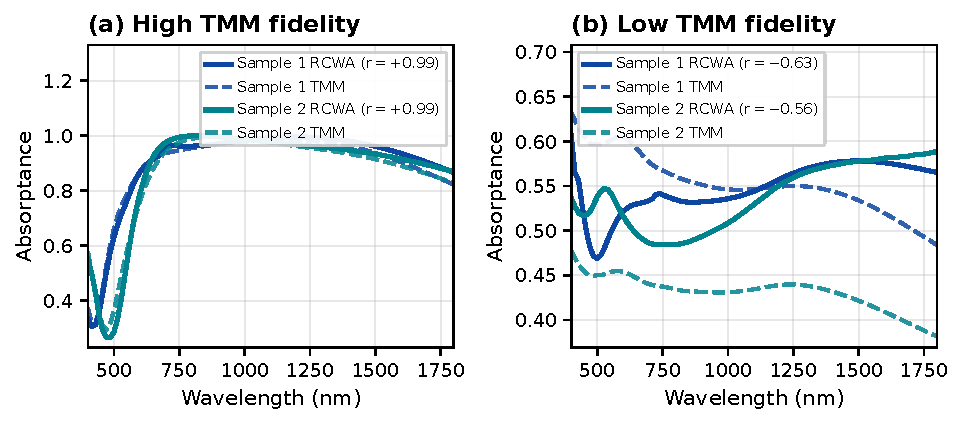
\includegraphics[width=\textwidth]{figures/Figure_2.pdf}
\caption{Representative TMM (dashed) vs.\ RCWA (solid) absorptance spectra for Structure~A; each panel shows two parameter sets, with each sample drawn in a distinct hue and the RCWA/TMM pair sharing that hue (legend lists the per-sample Pearson correlation $r$). (a)~High-fidelity cases ($r \approx 1.0$) where TMM closely tracks the RCWA cavity resonance. (b)~Low-fidelity cases ($r \approx -0.6$) where RCWA exhibits sharp resonance features that the planar TMM cannot reproduce.}
\label{fig:tmm_rcwa_spectra}
\end{figure}

All structures share a $100$\,nm Cr ground mirror, which keeps transmittance small: the per-structure mean transmittance is $T_\text{mean} < 0.7\%$ and the maximum over all RCWA samples is $T_\text{max} \lesssim 2.3\%$ (Supplementary Section~S12). We therefore model absorptance as $A = 1 - R$ with the surrogate predicting $R$ via sigmoid activation. Neglecting $T$ introduces an absolute error in $A$ of at most $T$, i.e.\ ${\sim}0.1$--$0.6\%$ on average and up to ${\sim}2.3\%$ for the worst-case sample---small relative to the reported MAE on $A$ at small training pools, though not negligible against the smallest MAE values at the largest pools.


\subsection{Neural Network Architecture}
\label{sec:architecture}

All surrogate models share a common ResNet backbone with 4 residual blocks (hidden dimension 256, LayerNorm, SiLU activation) to ensure fair comparison. The surrogate predicts reflectance $R$ via Sigmoid; absorptance is derived as $A = 1 - R$.

\subsubsection{Backbone: ResNet-256-4}

The backbone consists of a linear input projection followed by 4 residual blocks:
\begin{equation}
h^{(0)} = \text{SiLU}(\bm{W}_\text{in} \bm{x} + \bm{b}_\text{in}), \quad
h^{(\ell+1)} = h^{(\ell)} + \text{SiLU}\!\left(\text{ResBlock}^{(\ell)}(h^{(\ell)})\right)
\end{equation}
Each residual block contains two linear layers (hidden dimension 256) with LayerNorm and SiLU activation:
\begin{equation}
\text{ResBlock}(h) = \text{LN}_2\!\left(\bm{W}_2 \cdot \text{SiLU}\!\left(\text{LN}_1(\bm{W}_1 h + \bm{b}_1)\right) + \bm{b}_2\right)
\end{equation}

The output head maps the 256-dimensional representation to a scalar reflectance prediction:
\begin{equation}
R = \sigma\!\left(\bm{w}_\text{out} \cdot \text{SiLU}(\bm{W}_h \, h^{(4)} + \bm{b}_h) + b_\text{out}\right), \quad A = 1 - R
\end{equation}
where $\sigma$ denotes the sigmoid function.

\subsubsection{Input Representation}

Each training sample is a \emph{per-wavelength} data point: the input concatenates a normalized wavelength $\tilde{\lambda} \in [0,1]$ with the normalized geometric parameters (input dimension $d_\text{geo} = 1 + d$). A single geometry with $100$ wavelengths therefore yields $100$ training examples that share the same network weights, an implicit form of cross-wavelength regularization whose impact is examined in Section~\ref{sec:robustness_summary} (Architecture sensitivity). For statistical purposes, the effective sample size is $n$ (the number of unique geometries), since the $100$ wavelength rows per geometry are highly correlated.

Physics-augmented variants ($\Mphys$, $\Mtlphys$) append $n_\text{phys}$ physics features to the input. The added parameters affect only the first linear layer ($+0.78\%$ for Structure~A), too small to account for the $4$--$30\%$ relative MAE improvements (physics features, $\Mphys$ vs.\ $\Mzero$) we observe.


\subsection{Physics Feature Engineering}
\label{sec:features}

We derive wavelength-dependent features grouped into six categories: (i)~Fabry--P\'{e}rot \emph{cavity-resonance} phase $\varphi = 4\pi n_\text{cav}d\cos\theta_t/\lambda$ encoded as $\{\cos\varphi,\sin\varphi\}$ for each dielectric spacer; (ii)~\emph{fill fraction} ($f_\text{rect}{=}W_xW_y/P^2$, $f_\text{ring}$, $f_\text{disk}$, depending on geometry); (iii)~\emph{sub-wavelength ratios} $P/\lambda$ and feature-width-to-$\lambda$; (iv)~\emph{skin-depth ratio} $t_\text{metal}/\delta(\lambda)$ with $\delta = \lambda/(4\pi k_\text{metal})$; (v)~\emph{optical path} $n_\text{cav}d/\lambda$; and (vi)~\emph{angle and geometry} ($\cos\theta$, aspect ratio, $\alpha=4\pi k/\lambda$). Structure~A uses 17 features, B uses 13, and C uses 13 plus 5 polarization-specific features for the anisotropic TMM variant. All features are $z$-score normalized using TMM-Stage statistics held fixed during fine-tuning.


\subsection{Physics-Based Transfer Learning (PBTL) Framework}
\label{sec:pbtl}

PBTL consists of two stages. \textbf{Stage~1 (TMM generation and pre-training, ${\sim}108$\,s on a single GPU):} we generate $N_\text{TMM}=5{,}000$ random parameter samples drawn uniformly within the rectangular design ranges in Section~\ref{sec:structures} (without rejecting the minority of draws---e.g.\ fill fraction $>1$ in ${\sim}10$--$19\%$ of Structure~A/C samples---that fall outside the strict geometry manifold; because the identical pre-training library initializes every transfer variant, this does not bias the within-structure $\Mtl$-vs-$\Mzero$ comparison), compute their TMM spectra via EMA plus characteristic matrices (${\sim}19$\,s), and pre-train the ResNet for $500$ epochs (${\sim}88$\,s; lr $= 10^{-3}$, batch $2{,}048$; per-condition timings in Supplementary Section~S2); the per-wavelength training loss is the sum of MSE terms on the derived absorptance $A=1-R$ and on the predicted reflectance $R$, which reduces to approximately twice the reflectance MSE---exactly so for negligible transmittance, since the single sigmoid head predicts $R$ and $A=1-R$ is derived deterministically (the RCWA labels carry a small $T$, discussed below). \textbf{Stage~2 (RCWA fine-tuning):} the pre-trained weights are used as initialization and fine-tuned on $n$ RCWA samples for $1{,}000$ epochs at a lower learning rate (lr $=3\times10^{-4}$, batch $512$, cosine annealing, weight decay $10^{-4}$); the lower learning rate prevents catastrophic forgetting of the pre-trained knowledge. Physics features are included at both stages whenever the $\Mphys$ or $\Mtlphys$ variant is used, with normalization statistics fixed at Stage~1 to prevent distribution shift. For Structure~C, which is dual-polarization, two independent sigmoid heads predict $R_\text{TE}$ and $R_\text{TM}$ (absorptances derived as $A=1-R$ per polarization; transmittance is negligible and not predicted), and the loss is the sum of the four per-channel MSE terms on $(A_\text{TE}, R_\text{TE}, A_\text{TM}, R_\text{TM})$; details in Supplementary Section~S11.

\textbf{Hyperparameter selection.} Pre-training epochs ($500$) and Stage-2 epochs ($1{,}000$) were chosen so that validation MAE on a held-out $10\%$ TMM validation split ($500$ samples) flattens within $5\%$ of its minimum (saturation observed at ${\sim}300$ and ${\sim}600$ epochs respectively, $66\%$ buffer). The Stage-2 learning rate $3\times10^{-4}$---one third of Stage~1---was selected from the two-rate comparison ($10^{-3}$ vs.\ $3\times10^{-4}$) reported in Supplementary Section~S3: the lower rate gives a small but consistent validation advantage for $\Mtl$, consistent with reduced forgetting of the pre-trained knowledge. A direct check that this choice does not unfairly advantage $\Mtl$ over $\Mzero$ (which uses lr $=10^{-3}$) is reported in Supplementary Section~S3, where $\Mtl$ retains a $16$--$40\%$ improvement over $\Mzero$ even when both share lr $=10^{-3}$.

\textbf{Why supervise reflectance.} Predicting $R$ rather than $A$ directly is a deliberate design choice. Reflectance is bounded in $[0,1]$ and changes monotonically through the sigmoid output, which avoids the saturation behavior of an absorptance head near the absorption peaks where most of the spectral variation lives. Because transmittance is small across all three structures ($T_\text{mean} < 0.7\%$, $T_\text{max} \lesssim 2.3\%$; Supplementary Section~S12), the approximation $A = 1 - R$ introduces an absolute error in $A$ of at most $T$---on average ${\sim}0.1$--$0.6\%$, well below the reported MAE on $A$ (which ranges from ${\sim}1.7\%$ to ${\sim}8.4\%$ across structures and training sizes)---so the single-head formulation---predicting $R$ and deriving $A=1-R$, with the training loss summing the MSE on both quantities---behaves similarly to supervising two free outputs while halving the output dimensionality and stabilizing training (lower per-seed variance than an architecture with two independent $(A,R)$ output channels). For the small fraction of samples with the largest $T$ (up to ${\sim}2.3\%$), this residual term is no longer negligible against the smallest reported MAE values at the largest training pools.


\subsection{Experimental Design}
\label{sec:experimental}

\subsubsection{4-Way Model Comparison}

We compare four model variants to disentangle the contributions of physics features and transfer learning:
\begin{itemize}[leftmargin=*]
  \item $\Mzero$: Geometry-only input, trained from scratch on RCWA data.
  \item $\Mphys$: Geometry + physics features, trained from scratch.
  \item $\Mtl$: Geometry-only, pre-trained on TMM, fine-tuned on RCWA.
  \item $\Mtlphys$: Geometry + physics features, pre-trained on TMM, fine-tuned on RCWA.
\end{itemize}

Each configuration is evaluated at four RCWA training set sizes ($n \in \{50, 100, 200, 350\}$). The main 4-way comparison (Tables~\ref{tab:pbtl_a}--\ref{tab:pbtl_c}) uses 10 random seeds; due to computational constraints, control experiments use reduced seed counts: the multi-fidelity baseline experiments use 5 seeds, while the LR ablation, architecture ablation, and noise-injection experiments use 3 seeds per condition. All relative improvements reported in this paper are computed \emph{within} the same seed set; metrics are never compared across experiments with different seed counts. We report test MAE on absorptance (mean $\pm$ std over seeds). Fixed validation and test sets (50 geometries each) are reused across all model variants and training sizes. Exact split indices, seed values, and per-experiment sample lists are provided in the released code and data (see Code and Data Availability).

\subsubsection{Control Experiments}

\begin{itemize}[leftmargin=*]
  \item \textbf{Random baseline ($\Mrand$):} Pre-training on uniformly random absorptance spectra (no physics content) to verify that observed benefits arise from physics knowledge, not mere weight initialization or pre-training regularization.
  \item \textbf{TMM accuracy variation:} Systematic noise injection ($\sigma \in \{0, 0.05, 0.10, 0.15, 0.20, \infty\}$) into TMM training data to test the relationship between pre-training data quality and transfer learning benefit under controlled source-fidelity degradation.
  \item \textbf{TMM data size sensitivity:} $N_\text{TMM} \in \{500, 1{,}000, 2{,}000, 5{,}000\}$ to determine the minimum pre-training data requirement.
  \item \textbf{Learning rate ablation:} 4 LR combinations $\times$ 4 data sizes $\times$ 3 seeds $=$ 48 runs to rule out learning rate as a confound.
  \item \textbf{Architecture ablation:} ResNet-256-4 vs.\ a plain MLP (input projection to $256$ followed by three $256$-unit hidden layers and a $128$-unit head) comparison (3 seeds) to quantify backbone sensitivity.
  \item \textbf{Permutation feature importance:} 10-repetition permutation analysis to quantify individual physics feature contributions.
\end{itemize}


% =====================================================================
% 3. RESULTS
% =====================================================================
\section{Results}
\label{sec:results}

We organize the results as a three-step test of the PBTL hypothesis: first identifying where PBTL succeeds and fails across the three MIM structures, then explaining those contrasts through TMM--RCWA spectral fidelity, and finally testing the explanation under controlled and out-of-distribution (OOD; here, cross-material) conditions.

Concretely, we present the main 4-way model comparison across all three structures and synthesize the cross-structure trends (Sections~\ref{sec:results_a}--\ref{sec:cross_structure}). We then validate the mechanistic basis of PBTL through random-baseline and noise-injection experiments (Sections~\ref{sec:random_baseline}--\ref{sec:tmm_accuracy}). Finally, we assess robustness through a condensed ablation summary, a tighter test-set validation, and cross-material generalization (Sections~\ref{sec:robustness_summary}--\ref{sec:material_generalization}); detailed per-condition tables for each ablation are deferred to the Supplementary Information.

\subsection{Structure A: Asymmetric Dual-Cavity (10 Parameters)}
\label{sec:results_a}

Table~\ref{tab:pbtl_a} and Figure~\ref{fig:learning_curves} present the 4-way comparison on Structure~A (with learning curves for all three structures). The two transfer-learning variants dominate at every training size: pure weight transfer $\Mtl$ is the best model at the smaller pools ($n=50$ and $n=100$), while the combined $\Mtlphys$ is best at the larger pools ($n=200$ and $n=350$). In every cell the gap between $\Mtl$ and $\Mtlphys$ is small ($\leq 0.38$\,pp), and both clearly outperform the two from-scratch variants ($\Mzero$, $\Mphys$).

\begin{figure}[htbp]\centering
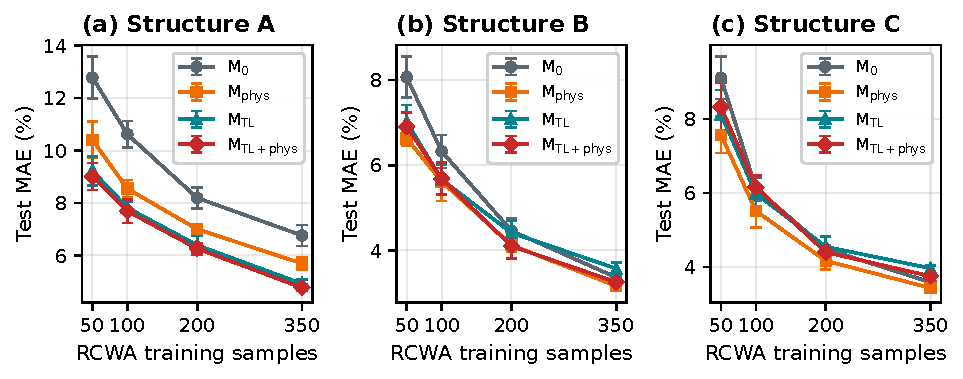
\includegraphics[width=\textwidth]{figures/Figure_3.pdf}
\caption{Learning curves (test MAE vs.\ RCWA training samples) for the 4-way model comparison across three MIM structures. Error bars show $\pm 1$ standard deviation over 10 seeds. Structure~A shows strong separation between the transfer-learning variants ($\Mtl$, $\Mtlphys$) and the from-scratch variants ($\Mzero$, $\Mphys$). For Structure~B the combined $\Mtlphys$ is best at every size, with physics features contributing a large share of the gain. For Structure~C pure weight transfer $\Mtl$ is the best model at every size and physics features contribute less than weight transfer, so physics features are not the primary contributor for that structure.}
\label{fig:learning_curves}
\end{figure}

\begin{table}[htbp]\centering\small
\caption{Test MAE (\%) on Structure A absorptance (mean $\pm$ std, 10 seeds; held-out test set $n_\text{test}=50$ per seed; tighter confidence-interval (CI) validation on a $99$-sample held-out test set is given in Section~\ref{sec:expanded_test}). Bold indicates best per row.}
\label{tab:pbtl_a}
\begin{tabular}{r cccc}\toprule
$n$ & $\Mzero$ & $\Mphys$ & $\Mtl$ & $\Mtlphys$ \\\midrule
50 & $8.36 \pm 0.63$ & $6.96 \pm 0.59$ & $\mathbf{4.21 \pm 0.49}$ & $4.59 \pm 0.42$\\
100 & $5.68 \pm 0.33$ & $4.89 \pm 0.33$ & $\mathbf{3.11 \pm 0.17}$ & $3.29 \pm 0.29$\\
200 & $3.93 \pm 0.35$ & $3.46 \pm 0.12$ & $2.39 \pm 0.11$ & $\mathbf{2.26 \pm 0.10}$\\
350 & $2.64 \pm 0.09$ & $2.52 \pm 0.07$ & $1.82 \pm 0.07$ & $\mathbf{1.79 \pm 0.04}$\\
\bottomrule
\end{tabular}
\end{table}

The relative MAE reduction of $\Mtlphys$ over $\Mzero$ ranges from \textbf{32.1\%} ($n=350$) to \textbf{45.1\%} ($n=50$). Notably, $\Mtlphys$ trained on only 50 RCWA samples ($\MAE = 4.59\%$) outperforms $\Mzero$ trained on 100 samples ($\MAE = 5.68\%$), demonstrating a $2\times$ data-efficiency gain.

\textbf{Disentangling contributions:} Physics features alone ($\Mphys$) reduce MAE by 5--17\%, while transfer learning alone ($\Mtl$) reduces it by 31--50\%. The combination ($\Mtlphys$) provides 32--45\% reduction---comparable to weight transfer alone---indicating that the two strategies are \emph{partially redundant}: both encode overlapping thin-film physics. Transfer learning captures this physics implicitly through weight initialization, while physics features provide it explicitly through input augmentation.

\textbf{Variance reduction:} the two TMM-pre-trained variants show markedly smaller seed-to-seed standard deviation than the from-scratch models: $\Mtlphys$ ranges $0.04$--$0.42\%$ and $\Mtl$ $0.07$--$0.49\%$, both well below $\Mzero$ ($0.09$--$0.63\%$). $\Mtlphys$ has the smallest std at three of the four training sizes; at $n=100$ pure weight transfer $\Mtl$ is marginally tighter ($0.17\%$ vs.\ $0.29\%$). TMM pre-training provides a stable initialization that reduces sensitivity to random seed selection.


\subsection{Structures B and C: Reduced but Positive Transfer}
\label{sec:results_b}

For Structures~B and~C, weight-level transfer ($\Mtl$ vs.\ $\Mzero$) is also positive at every training size, but the benefit is smaller than for~A and its ordering and magnitude differ from~A's (Tables~\ref{tab:pbtl_b} and~\ref{tab:pbtl_c}). For Structure~B the full transfer model $\Mtlphys$ is the best model at every $n$; for Structure~C pure weight transfer $\Mtl$ is best or tied-best. The degree of attenuation tracks the TMM--RCWA spectral fidelity in the operating band (Section~\ref{sec:cross_structure}): Structure~B, whose corrected TMM source is highly faithful (median $r=0.96$), retains a large benefit, while Structure~C, the lowest-fidelity case (median $r=0.65$, MAE $17\%$), retains the smallest.

\begin{table}[htbp]\centering\small
\caption{Test MAE (\%) on Structure B absorptance (mean $\pm$ std, 10 seeds; held-out test set $n_\text{test}=50$ per seed). Bold indicates best per row.}
\label{tab:pbtl_b}
\begin{tabular}{r cccc}\toprule
$n$ & $\Mzero$ & $\Mphys$ & $\Mtl$ & $\Mtlphys$ \\\midrule
50 & $5.50 \pm 0.52$ & $3.87 \pm 0.46$ & $3.50 \pm 0.18$ & $\mathbf{3.46 \pm 0.21}$\\
100 & $3.70 \pm 0.42$ & $2.82 \pm 0.23$ & $2.77 \pm 0.13$ & $\mathbf{2.74 \pm 0.20}$\\
200 & $2.56 \pm 0.17$ & $2.30 \pm 0.13$ & $2.21 \pm 0.05$ & $\mathbf{2.06 \pm 0.10}$\\
350 & $2.05 \pm 0.07$ & $1.77 \pm 0.07$ & $1.78 \pm 0.06$ & $\mathbf{1.65 \pm 0.04}$\\
\bottomrule
\end{tabular}
\end{table}

\begin{table}[htbp]\centering\small
\caption{Test MAE (\%) on Structure C with anisotropic TMM (mean $\pm$ std, 10 seeds; held-out test set $n_\text{test}=50$ per seed). Bold indicates best per row. The corrected-bounds regeneration yields $487$ reliable Structure-C samples, so the $n=350$ row draws its $350$ training geometries from the $387$-geometry pool available after the $50{+}50$ test/validation reservation.}
\label{tab:pbtl_c}
\begin{tabular}{r cccc}\toprule
$n$ & $\Mzero$ & $\Mphys$ & $\Mtl$ & $\Mtlphys$ \\\midrule
50 & $7.18 \pm 0.59$ & $5.89 \pm 0.58$ & $\mathbf{4.61 \pm 0.32}$ & $5.16 \pm 0.44$\\
100 & $4.61 \pm 0.30$ & $3.96 \pm 0.40$ & $\mathbf{3.41 \pm 0.13}$ & $3.68 \pm 0.17$\\
200 & $2.75 \pm 0.11$ & $2.60 \pm 0.18$ & $\mathbf{2.50 \pm 0.10}$ & $2.67 \pm 0.12$\\
350 & $2.12 \pm 0.09$ & $2.01 \pm 0.08$ & $\mathbf{1.91 \pm 0.04}$ & $2.05 \pm 0.09$\\
\bottomrule
\end{tabular}
\end{table}

\textbf{Structure~B: high-fidelity source, large retained benefit.} The ring--disk geometry supports Fano resonances arising from near-field coupling between the ring and disk---physics that the TMM\,+\,EMA source captures only approximately, since EMA collapses the two sub-elements into a single effective layer. Nonetheless, on the corrected materials and grid the broadband TMM--RCWA agreement is high: over the full 400--1800\,nm operating band the median shape correlation is $r = 0.96$ and the operating-band MAE is $8.9\%$ (Table~\ref{tab:tmm_fidelity}). A sub-band decomposition (Supplementary Section~S14) shows this agreement is not confined to any one region---median $r = 0.95$ in the visible and $0.97$--$1.00$ in the NIR, with MAE ${\sim}8$--$10\%$ in every sub-band. Because the source captures the broad thin-film envelope, weight-level transfer is positive at every training size and $\Mtlphys$ is the best model throughout; the analytically derived physics features (cavity phase, separate ring and disk fill fractions, sub-wavelength ratios) add further, partially redundant, structural information.

\textbf{Structure~C: lowest fidelity, smallest but still-positive benefit.} The 4-way comparison in Table~\ref{tab:pbtl_c} uses the \emph{anisotropic} TMM variant (Section~\ref{sec:methods}), which computes separate TE and TM responses and supplies five polarization-specific physics features. A planar EMA source model cannot fully represent geometry-dependent TE/TM splitting, so Structure~C has the lowest TMM--RCWA fidelity of the three (median $r = 0.65$, operating-band MAE $= 16.9\%$; Table~\ref{tab:tmm_fidelity}). Consistent with the fidelity--benefit relationship, Structure~C retains the smallest weight-transfer benefit, but it remains \emph{positive} at every training size---$\Mtl$ vs.\ $\Mzero$ falls from $+36\%$ at $n=50$ to $+9.7\%$ at the maximum pool---and $\Mtl$ is the best or tied-best model throughout (the corrected-bounds regeneration yields $487$ reliable samples, so the $n=350$ row draws $350$ training geometries from the $387$-geometry pool available after the $50{+}50$ test/validation reservation). The isotropic TMM replica in Section~\ref{sec:tmm_accuracy} shows a monotone fidelity--benefit decrease under a simpler scalar-output protocol on this structure.

\textbf{Common pattern: positive transfer graded by source fidelity.} For both structures weight-level transfer ($\Mtl$ vs.\ $\Mzero$) is positive at every training size---for~B from $+36\%$ ($n=50$) to $+13\%$ ($n=350$), for~C from $+36\%$ to $+9.7\%$---and a transfer variant ($\Mtlphys$ for~B, $\Mtl$ for~C) is the best model in every cell. The benefit is smaller than for Structure~A and shrinks as the fine-tuning pool grows (the $\Mzero$ baseline itself improves with more data), but it never turns negative for any of the three real structures. Crucially, the magnitude is ordered by the absolute operating-band MAE rather than by shape correlation $r$ alone: Structure~B has the \emph{highest} correlation ($r=0.96$) yet a smaller benefit than~A, whereas the MAE ordering ($7.9$, $8.9$, $16.9\%$ for A, B, C) matches the benefit ordering (A\,$>$\,B\,$>$\,C). Genuine negative transfer emerges only once source fidelity falls below a structure-dependent point---near zero for the high-fidelity Structure~A, but at moderate degradation ($\sigma=0.10$) for the lower-fidelity Structures~B and~C---which we demonstrate by controlled degradation in Section~\ref{sec:tmm_accuracy}.


\subsection{Cross-Structure Analysis}
\label{sec:cross_structure}

\begin{table}[htbp]\centering\small
\caption{Cross-structure summary of best-performing model and relative MAE improvement over the geometry-only baseline $\Mzero$ at $n=350$ RCWA training samples. The three structures span qualitatively different dominant physics, yielding a fidelity-graded transfer benefit that is largest for Structure~A and smallest for Structure~C.}
\label{tab:summary_350}
\begin{tabular}{lcccc}\toprule
\textbf{Structure} & \textbf{Params} & $\Mzero$ MAE & \textbf{Best Model} & \textbf{Improvement}\\\midrule
A (Dual-Cavity)       & 10 & 2.64\% & $\Mtlphys$ (1.79\%) & \textbf{32.1\%}\\
B (Ring-Disk Fano)    & 8  & 2.05\% & $\Mtlphys$ (1.65\%) & \textbf{19.7\%}\\
C (Dual-Polarization) & 7  & 2.12\% & $\Mtl$ (1.91\%) & \textbf{9.7\%}\\\bottomrule
\end{tabular}
\end{table}

The results show a consistent pattern: \textbf{TMM pre-training benefit is strongly associated with operating-band TMM--RCWA spectral fidelity (shape and amplitude jointly), rather than with design-space dimensionality per se}. Structure~A, with the lowest operating-band MAE---i.e.\ the highest amplitude fidelity (MAE $=7.9\%$, median $r=0.83$)---benefits most from transfer learning despite having the most parameters (10). Structures~B (median $r=0.96$, MAE $=8.9\%$) and C (median $r=0.65$, MAE $=16.9\%$) retain positive but progressively smaller weight-level TL benefit as operating-band amplitude error grows---regardless of their lower dimensionality (8 and 7 parameters). In our three structures, parameter count and operating-band TMM fidelity happen to be confounded, so we cannot separate their effects; with only $N=3$ structures we do not claim that fidelity is causal and dimensionality coincidental, only that the benefit ordering follows operating-band fidelity in these cases and that more complex structures here tended to have more dominant thin-film physics that TMM captures well. Physics features, by contrast, benefit all structures and are governed by a different mechanism (explicit feature engineering rather than implicit weight transfer).

\textbf{TMM fidelity explains cross-structure variation.} We computed the TMM--RCWA spectral MAE and per-sample Pearson correlation $r_i$ (across the 100 wavelengths for Structures~A and B, and across the 200 concatenated TE+TM spectral points for Structure~C) on up to 500 shared parameter sets per structure ($500$, $499$, $500$ for A, B, and~C) (Table~\ref{tab:tmm_fidelity}).

\textbf{Two fidelity views, one consistent metric.} The cross-structure metric (Table~\ref{tab:tmm_fidelity}) and the noise-injection metric (Table~\ref{tab:tmm_noise}, Section~\ref{sec:tmm_accuracy}) now use the \emph{same} estimator---median per-sample Pearson $r$ and median per-sample MAE over wavelengths in the operating band. For Structure~A the noise-experiment shape value at zero noise ($r=0.77$ on the 50-geometry test split) is close to the cross-structure value ($r=0.83$ on the full reliable pool), the small gap reflecting the test subsample. The cross-structure ranking ($A > B > C$ by operating-band MAE) matches the $\Mtl$-vs-$\Mzero$ benefit ranking ($A:\,+31.3\%$, $B:\,+13.5\%$, $C:\,+9.7\%$) descriptively at $N=3$; the controlled Structure-A noise experiment then supplies the primary single-structure evidence, where---consistently with the cross-structure picture---the operating-band MAE predicts the benefit far better than the shape correlation $r$ ($|$Pearson$|=0.98$ vs.\ $0.81$, Section~\ref{sec:tmm_accuracy}). All three structures are evaluated on the unified $400$--$1800$\,nm simulation grid (Section~\ref{sec:rcwa_methods}), so Table~\ref{tab:tmm_fidelity} compares them on a common broadband band; a visible ($400$--$780$\,nm) sub-band breakdown for B and C, reported in Supplementary Section~S14, shows the band-dependent behavior of the EMA used by TMM and supports the joint $r$-and-MAE diagnostic.

\begin{table}[htbp]\centering\small
\caption{TMM fidelity and transfer learning benefit by structure. TMM--RCWA accuracy is the \emph{median} of the per-sample spectral correlation $r$ and per-sample operating-band absolute MAE over the matched parameter sets ($500$, $499$, $500$ for A, B, and~C) at $n_\text{RCWA}=350$. For Structure~C the per-sample $r$ and MAE are computed over the 200 concatenated TE+TM spectral points (100 wavelengths $\times$ 2 polarizations). \textit{Best Gain} is defined as $1 - \mathrm{MAE}(M_\text{best})/\mathrm{MAE}(\Mzero)$, where $M_\text{best}$ is the lowest-MAE variant among $\{\Mphys, \Mtl, \Mtlphys\}$ for that structure (listed in the \textit{Best Model} column). \textit{Best Gain} (best model vs.\ $\Mzero$) is distinct from---and larger than---the weight-level transfer benefit ($\Mtl$ vs.\ $\Mzero$; $+31.3\%$, $+13.5\%$, $+9.7\%$ for A, B, C at $n=350$) emphasized in the text and Figure~\ref{fig:tmm_fidelity}, which isolates the contribution of the pre-trained weights alone. All percentage reductions in this paper are computed from unrounded mean MAE; recomputing them from the displayed two-decimal MAE values may differ by ${\leq}0.3$\,pp.}
\label{tab:tmm_fidelity}
\begin{tabular}{lccccc}\toprule
\textbf{Structure} & \textbf{TMM MAE} & \textbf{Mean $r$} & \textbf{Median $r$} & \textbf{Best Gain} & \textbf{Best Model}\\\midrule
A (Dual-Cavity)       & 7.9\% & 0.69 & 0.83 & \textbf{32.1\%} & $\Mtlphys$\\
B (Ring-Disk)         & 8.9\% & 0.88 & 0.96 & 19.7\% & $\Mtlphys$\\
C (Dual-Polarization) & 16.9\% & 0.53 & 0.65 & 9.7\% & $\Mtl$\\\bottomrule
\end{tabular}
\end{table}

Structure~A has the lowest operating-band TMM--RCWA MAE---i.e.\ the highest amplitude fidelity (MAE $= 7.9\%$, median $r = 0.83$; Structure~B has a higher median $r$ of $0.96$ but a larger MAE of $8.9\%$)---and the strongest weight-transfer benefit. Structures~B (MAE $= 8.9\%$, median $r = 0.96$) and C (MAE $= 16.9\%$, median $r = 0.65$) retain positive but progressively smaller weight-level transfer at $n_\mathrm{RCWA}=350$ ($\Mtl$ vs.\ $\Mzero$ benefit: $+13.5\%$ for B, $+9.7\%$ for C; see Tables~\ref{tab:pbtl_b}--\ref{tab:pbtl_c}). The cross-structure ranking is descriptively monotonic across all three structures ($A > B > C$ in $\Mtl$ benefit at $N=3$, ordered by operating-band MAE; the median-$r$ ordering $B > A > C$ mis-ranks the benefit); the controlled noise-injection experiment on Structure~A (Section~\ref{sec:tmm_accuracy}), where the operating-band MAE predicts the benefit far better than shape correlation~$r$ ($|$Pearson$|=0.98$ vs.\ $0.81$; Spearman $\rho=\pm1.0$), provides the primary controlled evidence for the fidelity--benefit relationship. The empirical relationship between TMM accuracy and weight-transfer benefit, visualized in Figure~\ref{fig:tmm_fidelity}, supports a practical \textbf{pre-screening procedure}: practitioners can estimate expected PBTL benefit by evaluating TMM--RCWA spectral fidelity on a small pilot set before committing to expensive full data collection. The corrected values show, however, that shape correlation $r$ alone is insufficient: Structure~B has the \emph{highest} $r$ ($0.96$) yet a smaller benefit than~A, and the benefit ordering follows the absolute operating-band MAE (A\,$<$\,B\,$<$\,C) rather than $r$ (B\,$>$\,A\,$>$\,C). We therefore recommend a \textbf{joint pre-screening criterion} combining median $r$ and median MAE in the target operating band rather than relying on $r$ alone.

\textbf{Pilot-set validation.} To verify that the diagnostic is reliable at small sample sizes, we performed a bootstrap subsampling analysis on all $500$ evaluated Structure~A geometries with finite TMM--RCWA fidelity (median per-sample $r=0.83$). The per-sample median Pearson $r$ was computed for random subsets of size $n_\text{pilot} \in \{10, 20, 50, 100\}$ over 1{,}000 bootstrap repetitions. At $n_\text{pilot} = 20$ the estimated median $r = 0.81 \pm 0.08$ (95\% CI: $[0.61, 0.92]$), with $99.7\%$ of replicates retaining a median $r > 0.5$ (rising to $100\%$ by $n_\text{pilot}=50$); at $n_\text{pilot} = 50$ the precision improves to $\pm 0.05$ (95\% CI: $[0.70, 0.90]$). The bias relative to the full-pool reference ($r = 0.83$) is $< 0.02$ at $n_\text{pilot} = 20$ and $< 0.01$ at $n_\text{pilot} = 50$. These Structure-A results demonstrate stable pilot estimation of the correlation component. Because the corrected analysis identifies the absolute operating-band MAE---rather than shape correlation---as the dominant predictor of the transfer benefit, we applied the identical bootstrap to the MAE component and extended it to Structures~B and C. The per-sample median MAE is recovered with small bias and tightening precision: Structure~A gives $8.2 \pm 1.3\%$ at $n_\text{pilot}=20$ and $7.9 \pm 0.7\%$ at $n_\text{pilot}=50$ (full-pool reference $7.9\%$); Structure~B, $9.2 \pm 1.6\%$ and $9.0 \pm 0.9\%$ (reference $8.9\%$); and Structure~C, $16.9 \pm 2.1\%$ and $16.8 \pm 1.5\%$ (reference $16.9\%$); the absolute bias is $<0.3$\,pp at $n_\text{pilot}=20$ and $<0.2$\,pp at $n_\text{pilot}=50$ for all three. The correlation component is likewise stable for B and C (median-$r$ bias $<0.03$ at $n_\text{pilot}=20$ and $<0.01$ at $n_\text{pilot}=50$). The practical resolution of the pilot is set by the inter-structure fidelity gap: the low-fidelity structure (C, MAE\,$\approx 17\%$) is cleanly separated from the high-fidelity pair by $n_\text{pilot}\geq 20$ (the three structures' MAE confidence intervals still overlap at $n_\text{pilot}=10$), whereas the $\sim 1$\,pp MAE gap between the two high-fidelity structures (A vs.\ B) is comparable to the pilot scatter (of order one standard deviation even at $n_\text{pilot}=100$) and is not reliably resolved by a single small pilot. A small ($\leq 50$-geometry) pilot therefore estimates both components of the joint criterion (Section~\ref{sec:guidelines}) with quantified precision and reliably flags low-fidelity transfer sources---both components must be checked on that pilot before a go/no-go decision---but it should not be over-interpreted as finely ranking sources of already-similar fidelity. This bootstrap operates on the per-sample fidelity of all evaluated geometries ($500$, $499$, $500$ for Structures~A, B, and~C); restricting it to the reliability-filtered training pools ($499$, $498$, $487$) changes no reported median. It is reproduced by \texttt{pilot\_bootstrap\_redesign.py} in the released code. The pilot computation itself requires only minutes of additional GPU time on top of the standard RCWA generation.

\textbf{Statistical significance.} All pairwise comparisons (10 seeds) were tested using paired $t$-tests. For Structure~A, $\Mtlphys$ vs.\ $\Mzero$ is significant at every training size ($p < 10^{-6}$, pooled Cohen's $d > 6$). The two transfer variants $\Mtl$ and $\Mtlphys$ are near-equivalent and neither dominates: $\Mtl$ is the lower-MAE model at the small pools (significantly so at $n=50$, paired $p=0.003$) and $\Mtlphys$ at the large pools (significantly so at $n=200$, $p=0.003$), while the $n=100$ and $n=350$ differences are not significant ($p=0.12$ and $p=0.37$)---consistent with the per-row best model in Table~\ref{tab:pbtl_a}. For the physics-feature claim ($\Mphys$ vs.\ $\Mzero$), $11$ of the $12$ conditions (3 structures $\times$ 4 training sizes) remain significant after Holm--Bonferroni correction across the family (Welch's $t$-test, Cohen's $d \in [0.93, 3.94]$); the sole exception is Structure~C at $n=200$ (Welch $p=0.055$, $d=0.93$, Holm-adjusted $p=0.055$), which is marginal. The mean physics-feature MAE reduction is nonetheless positive in all $12$ conditions, supporting the abstract claim that physics features reduce error across all three tested structures. For Structures~B and~C a transfer variant is the best model at every size ($\Mtlphys$ for~B, $\Mtl$ for~C; Tables~\ref{tab:pbtl_b}--\ref{tab:pbtl_c}), though its margin over $\Mphys$ is small at the largest training pools.

\begin{figure}[htbp]\centering
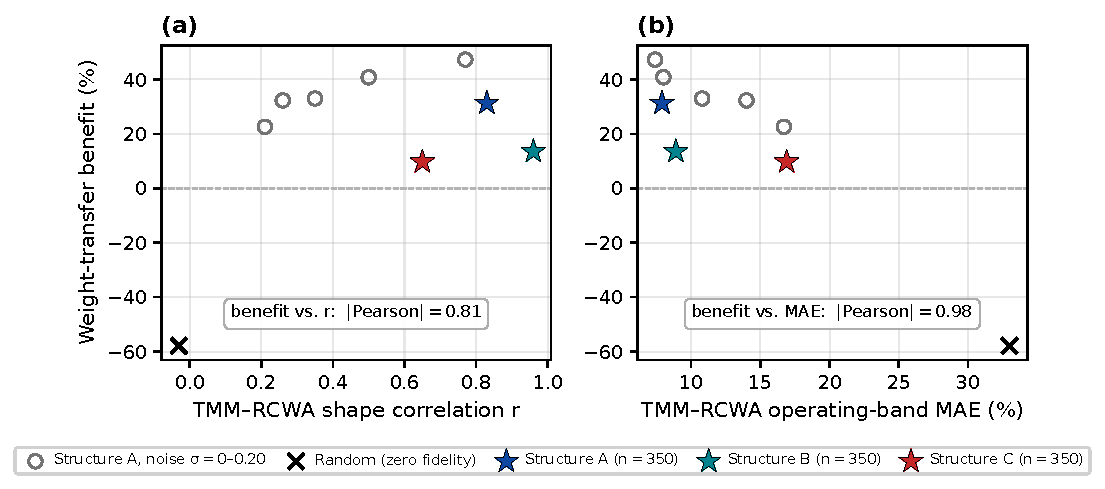
\includegraphics[width=\textwidth]{figures/Figure_4.pdf}
\caption{TMM--RCWA fidelity vs.\ weight-transfer benefit, plotted against (a)~the shape correlation $r$ and (b)~the operating-band absolute MAE. Benefit is $1-\mathrm{MAE}(\Mtl)/\mathrm{MAE}(\Mzero)$ (for the noise points, $\Mtl^{\sigma}$ vs.\ $\Mzero$). Gray circles: controlled noise-injection conditions on Structure~A ($\sigma=0,0.05,0.10,0.15,0.20$; RCWA $n=100$); black~X: random (zero-fidelity) source. Coloured stars: cross-structure points (A, B, C) at $n=350$, using the TMM--RCWA median per-sample $r$ and operating-band MAE of Table~\ref{tab:tmm_fidelity}. Both panels use the same median per-sample fidelity definition. The operating-band MAE (panel~b) predicts the benefit markedly better than the shape correlation (panel~a)---descriptive Pearson $|r|=0.98$ vs.\ $0.81$ over the six Structure-A conditions---and the cross-structure stars follow the MAE ordering ($A<B<C$) but \emph{not} the $r$ ordering ($B>A>C$), so the amplitude component, not shape correlation alone, orders the benefit here. The noise circles ($n_\text{RCWA}=100$) and cross-structure stars ($n=350$) are overlaid for descriptive context, not direct comparison---they differ in RCWA training-set size and in whether the source degradation is controlled (noise) or structure-intrinsic---so the recommended pre-screening rule is the joint $r$-and-MAE diagnostic of Section~\ref{sec:guidelines}. All three structures and the noise conditions are evaluated on the common $400$--$1800$\,nm grid (Section~\ref{sec:rcwa_methods}).}
\label{fig:tmm_fidelity}
\end{figure}


%--- Mechanistic Validation ---
\subsection{Random Pre-training Baseline}
\label{sec:random_baseline}

To rule out that the observed TL benefit reflects mere regularization rather than physics knowledge, we compared $\Mtl$ against $\Mrand$, pre-trained on uniformly random absorptance spectra. $\Mrand$ provides essentially no benefit---its MAE stays within ${\sim}6\%$ of $\Mzero$ at every training size, i.e.\ statistically indistinguishable from training from scratch---whereas $\Mtl$ reduces MAE by $20$--$50\%$ on Structure~A (this random-baseline seed set); the $0.5$--$4.3$\,pp gap between $\Mtl$ and $\Mrand$ (largest at small $n$) confirms that TMM pre-training transfers genuine physics content, not arbitrary weight initialization. Full per-seed table is reported in Supplementary Section~S1.


\subsection{TMM Accuracy--Transfer Learning Benefit Correlation}
\label{sec:tmm_accuracy}

To test the mechanistic relationship between TMM fidelity and transfer learning benefit, we systematically degraded TMM pre-training data through noise injection ($\sigma = 0$ to $\infty$), creating $N=6$ controlled experimental conditions within a single structure (A). By varying TMM data quality while keeping the RCWA fine-tuning dataset identical, pre-training quality serves as the sole independent variable in this controlled analysis.

\begin{table}[htbp]\centering\small
\caption{TMM source-fidelity degradation experiment (Structure~A, RCWA $n=100$, 3 seeds per condition). Both the shape fidelity (median per-sample Pearson $r$) and the amplitude fidelity (TMM--RCWA operating-band MAE) of the noisy source are reported against the transfer benefit.}
\label{tab:tmm_noise}
\begin{tabular}{cccccr}\toprule
\textbf{Level} & \textbf{Noise $\sigma$} & \textbf{TMM $r$ (shape)} & \textbf{TMM MAE (\%)} & $\Mtl$ \textbf{MAE (\%)} & \textbf{TL Benefit}\\\midrule
0 & 0.00 & $0.77$ & $7.4$ & $3.05 \pm 0.12$ & $+47.3\%$\\
1 & 0.05 & $0.50$ & $8.0$ & $3.42 \pm 0.18$ & $+40.8\%$\\
2 & 0.10 & $0.35$ & $10.8$ & $3.87 \pm 0.13$ & $+33.0\%$\\
3 & 0.15 & $0.26$ & $14.0$ & $3.91 \pm 0.16$ & $+32.3\%$\\
4 & 0.20 & $0.21$ & $16.7$ & $4.48 \pm 0.19$ & $+22.6\%$\\
5 & $\infty$ (random) & $-0.03$ & $33.0$ & $9.13 \pm 0.58$ & $-57.9\%$\\
\bottomrule
\end{tabular}
\end{table}

The $\Mzero$ baseline for this experiment is $5.78 \pm 0.33\%$ (3 seeds). Transfer learning benefit is computed as $(1 - \MAE_\text{TL} / \MAE_\text{M0}) \times 100\%$, using the matched 3-seed $\Mzero$ as the denominator to ensure a fair within-experiment comparison. The TMM $r$ and TMM MAE columns are, respectively, the median per-sample Pearson correlation over wavelengths and the median per-sample absolute error in the operating band on the 50-geometry RCWA test set---the same fidelity definition used in Table~\ref{tab:tmm_fidelity} and the Structure-B/C replicas (replacing an earlier pooled-flatten Pearson).

\textbf{Statistical summary.} The five physics-based noise conditions are not independent replicates: the noise levels are nested (the same Gaussian draws rescaled by $\sigma$), all conditions share a single TMM pre-training data pool, and all benefit values share the common 3-seed $\Mzero$ denominator. We therefore present the following as \emph{descriptive} summaries of a controlled, ordered experiment rather than as formal hypothesis tests:
\begin{itemize}[leftmargin=*]
  \item \textbf{Primary ($N=6$, all ordered conditions including the zero-fidelity control):} the benefit decreases monotonically with both fidelity measures (Spearman $\rho = \pm 1.0$). Over the full range including the zero-fidelity control, the operating-band absolute MAE is a markedly stronger linear predictor of the benefit (Pearson $|r| = 0.98$, parametric $p = 5\times10^{-4}$) than the shape correlation $r$ ($0.81$): the shape correlation saturates as the source degrades, whereas the MAE tracks the benefit's collapse, reproducing within a single controlled structure the cross-structure finding that \emph{amplitude} error is the strongest observed predictor of the transfer benefit in these experiments. Because of the dependence structure described above, these $p$-values are descriptive.
  \item \textbf{Robustness ($N=5$, excluding the zero-fidelity control):} excluding the zero-fidelity control the two measures are comparably strong (MAE Pearson $|r| = 0.95$, $p = 0.013$; shape-$r$ Pearson $0.94$; Spearman $\rho = \pm 1.0$ for both), so the relationship does not hinge on the random extreme. The same dependence caveat applies; all summaries are descriptive.
\end{itemize}

This experiment yields four observations. The transfer benefit decreases monotonically with source fidelity (Spearman $\rho = \pm 1.0$), even excluding the random extreme, and positive transfer ($+23\%$) is maintained even at $\sigma = 0.20$ (operating-band MAE $16.7\%$, shape $r = 0.21$). Random pre-training (MAE $33\%$, $r \approx 0$) drives catastrophic negative transfer ($-58\%$) at this small-$n$ operating point, although the 10-seed random baseline (Section~\ref{sec:random_baseline}) separately shows that random pre-training is, on average, statistically indistinguishable from training from scratch. Finally, the operating-band absolute MAE predicts the benefit better than the shape correlation $r$ alone ($|\text{Pearson}| = 0.98$ vs.\ $0.81$ over the full range), an internal single-structure confirmation that amplitude error is the strongest observed predictor of the benefit, consistent with the cross-structure picture in Section~\ref{sec:cross_structure}.

The cross-structure analysis (Section~\ref{sec:cross_structure}) offers limited, descriptive support consistent with this relationship: across the three structures the benefit is ordered by operating-band MAE, but with only $N=3$ points and a weak three-structure linear fit this is suggestive rather than independent confirmation, and the controlled single-structure noise experiment remains the primary evidence.

\paragraph{Replication on Structures B and C.} To test whether the controlled fidelity--benefit relationship extends beyond Structure~A, we applied the same noise-injection protocol to Structures~B and~C, using a single-polarization TMM target (for~C, the isotropic variant) to match the per-wavelength scalar formulation of the Structure-A experiment (four noise levels $\sigma = 0$, 0.10, 0.20, $\infty$; 3 seeds; $n_\text{rcwa}=100$; these are separate scalar experiments from the main 4-way results in Tables~\ref{tab:pbtl_b}--\ref{tab:pbtl_c}). Table~\ref{tab:tmm_noise_BC} reports the outcome.

\begin{table}[htbp]\centering\small
\caption{Noise-injection replica on Structures~B and~C using a single-polarization TMM target (for~C, the isotropic variant) matched to the Structure-A scalar protocol (RCWA $n=100$, 3 seeds per condition, 2{,}000 fresh TMM samples per level). $\Mzero$ baselines: B $3.70\%$, C $3.47\%$. The fidelity--benefit Pearson is $0.99$ (B) and $0.97$ (C) over the four ordered conditions. Benefit $=(1-\MAE_\text{TL}/\MAE_\text{M0})\times100\%$. The per-level TMM--RCWA accuracy $r$ is the median per-sample Pearson over the full reliable pool, and the TMM library is drawn from the fixed design bounds. The B/C noise replicas use a per-seed held-out test split (vs.\ the single fixed split of the main PBTL and ablation experiments), so the seed dispersion includes a small test-split component; this does not bias the within-level $\Mtl$-vs-$\Mzero$ comparison.}
\label{tab:tmm_noise_BC}
\begin{tabular}{llccr}\toprule
\textbf{Struct.} & \textbf{Noise $\sigma$} & \textbf{TMM Acc.\ ($r$)} & $\Mtl$ \textbf{MAE (\%)} & \textbf{TL Benefit}\\\midrule
B & 0.00               & $+0.96$ & $3.07 \pm 0.15$ & $+17.1\%$\\
B & 0.10               & $+0.77$ & $4.64 \pm 0.19$ & $-25.2\%$\\
B & 0.20               & $+0.52$ & $5.87 \pm 0.34$ & $-58.6\%$\\
B & $\infty$ (random)  & $+0.00$ & $11.74 \pm 0.34$ & $-216.9\%$\\\midrule
C & 0.00               & $+0.88$ & $2.90 \pm 0.31$ & $+16.3\%$\\
C & 0.10               & $+0.54$ & $4.54 \pm 0.28$ & $-31.1\%$\\
C & 0.20               & $+0.34$ & $5.88 \pm 0.27$ & $-69.6\%$\\
C & $\infty$ (random)  & $+0.01$ & $9.68 \pm 0.42$ & $-179.2\%$\\\bottomrule
\end{tabular}
\end{table}

The controlled experiment now reproduces the fidelity--benefit \emph{collapse} on all three structures: under the same fine-tuning protocol as Structure~A, the benefit on Structures~B and~C falls monotonically as the source degrades, with descriptive fidelity--benefit Pearson $r=0.99$ (B) and $0.97$ (C) over the four ordered conditions (Table~\ref{tab:tmm_noise_BC}), alongside $r=0.81$ for the six-level Structure-A sweep. The informative difference is the \emph{rate} of collapse. The lower-fidelity Structures~B and~C cross into negative transfer already at $\sigma=0.10$ ($-25\%$ for B, $-31\%$ for C), whereas the higher-fidelity Structure~A remains positive through $\sigma=0.20$ ($+23\%$); at zero fidelity all three reach catastrophic negative transfer ($-58\%$, $-217\%$, $-179\%$ for A, B, C, the larger B/C magnitudes reflecting their smaller $\Mzero$ denominators). This is consistent with the finding that amplitude (MAE) error orders the benefit (the B/C replicas report the source shape $r$ in Table~\ref{tab:tmm_noise_BC}; their larger clean operating-band MAE is read from Table~\ref{tab:tmm_fidelity}): a source whose clean operating-band MAE is already large (B $8.9\%$, C $16.9\%$) is pushed below the useful threshold by a smaller perturbation than the high-fidelity Structure~A ($7.9\%$), so the Structure-B/C replicas are descriptively consistent with the Structure-A gradient rather than merely confirming its zero-fidelity endpoint. These replicas each rest on only four ordered noise levels per structure and use a different per-seed held-out test split from the main experiments (Table~\ref{tab:tmm_noise_BC} caption), so they are descriptive evidence rather than a formal test. Taken together with the cross-structure operating-band MAE ordering (Section~\ref{sec:cross_structure}), they are consistent with the \emph{amplitude} of the source error---rather than its shape correlation alone---being the quantity that tracks the transfer benefit in these experiments.


%--- Robustness and Generalization ---
\subsection{Robustness and Ablation Summary}
\label{sec:robustness_summary}

A series of ablations confirms that, for the high-fidelity Structure~A case, weight-level TMM transfer is a genuine source of PBTL's gain rather than an artifact of the specific design choices made for the main 4-way comparison. Full tables and per-condition standard deviations are reported in Supplementary Information.

\textbf{Pre-training data size:} A sweep of $N_\text{TMM}\!\in\!\{500,\,1{,}000,\,2{,}000,\,5{,}000\}$ shows the weight-transfer benefit grows monotonically with pre-training data and does not saturate through $5{,}000$ samples: in the data-scarce regime ($n_\text{RCWA}{=}100$) it rises from ${\sim}{+}26\%$ at $500$ TMM samples to ${\sim}{+}45\%$ at $5{,}000$, at $<\!1\%$ computational overhead (Supplementary Section~S2).

\textbf{Learning rate confound:} A full factorial $48$-run sweep ($2$ models $\times$ $2$ LRs $\times$ $4$ sizes $\times$ $3$ seeds) shows $\Mtl$ retains a positive matched-LR improvement over $\Mzero$---$+16$ to $+40\%$ for Structure~A, $+11$ to $+26\%$ for B, and a marginal $0$ to $+8\%$ for the low-fidelity C, with both models sharing $\text{lr}{=}10^{-3}$---ruling out the lower fine-tuning LR as the cause (Supplementary Section~S3).

\textbf{Backbone capacity:} For the high-fidelity Structure~A case, replacing the ResNet-$256$-$4$ (${\sim}567$\,K parameters) with a plain MLP (${\sim}233$\,K) still yields a sizable TL gain ($21$--$53\%$ across the tested sizes), indicating that PBTL is not merely compensating for ResNet capacity in this case. The same ablation exposes an architecture caveat for lower-fidelity Structures~B and~C, where, in the isotropic single-output Structure-C variant used for this ablation (whose $\Mzero$ baseline differs from the main dual-polarization result, so its cells are not directly comparable to Table~\ref{tab:pbtl_c}), both the MLP and---marginally---the ResNet can dip slightly negative (${\approx}-1\%$) at the largest training sizes; this caveat is reported in Supplementary Section~S4.

\textbf{Feature importance:} Permutation analysis on $\Mphys$ ranks cavity-phase features (${\sim}37\%$ of total importance) and fill fraction (${\sim}23\%$) as the two dominant feature categories---about $60\%$ together---validating the Fabry--P\'{e}rot interpretation of the dominant absorption mechanism (Supplementary Section~S5; Figure~\ref{fig:feature_importance}).

\textbf{TMM-as-input baseline:} Providing the scalar TMM absorptance directly as an additional input feature ($M_\text{TMM-in}$) improves over $\Mzero$ only marginally ($0$--$11\%$, vanishing or slightly negative at the larger pools $n{=}200,350$) and remains far behind $\Mtlphys$. This confirms that the bulk of the gain comes from the \emph{distributed} weight initialization rather than from any single TMM scalar input (Supplementary Section~S6).

\textbf{Multi-fidelity comparison:} Against three classical baselines (linear correction, residual NN, Co-Kriging~\cite{kennedy2000predicting}) and a deep composite multi-fidelity NN~\cite{meng2020composite}, $\Mtlphys$ achieves the lowest MAE at all training sizes---$28$--$38\%$ lower than the strongest (lowest-MAE) baseline at each size, and up to $76\%$ lower than linear correction. Importantly, expanding the Co-Kriging TMM budget from $500$ to $2{,}000$ via a sparse variational Gaussian process (GP)~\cite{hensman2015scalable} did not close the gap to $\Mtlphys$ in this sparse-GP variant, indicating the advantage is not explained merely by the Co-Kriging TMM-data budget (Supplementary Section~S7).

\textbf{Architecture sensitivity:} Replacing the per-wavelength formulation with a Full-Spectrum ResNet (output $\in\mathbb{R}^{100}$ per parameter set) yields uniformly higher MAE ($11$--$38\%$ worse than per-wavelength, depending on model and training size) but a comparable PBTL benefit ($+24.6\%$ to $+48.0\%$). The two design choices are thus complementary and multiplicative rather than substitutable (Supplementary Section~S8).

\begin{figure}[htbp]\centering
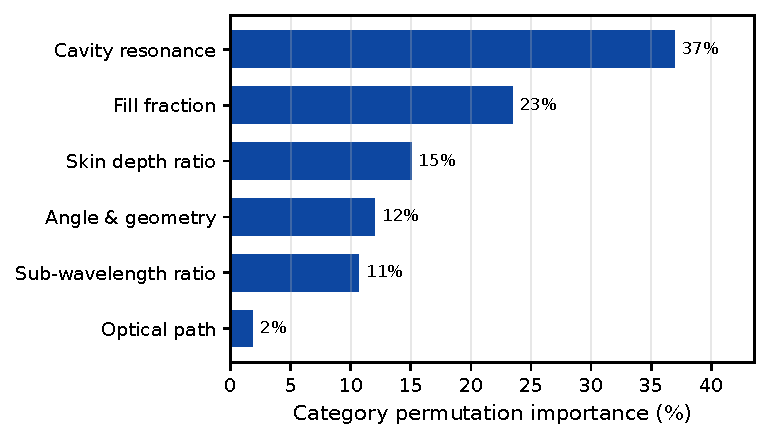
\includegraphics[width=0.77\textwidth]{figures/Figure_5.pdf}
\caption{Category-level permutation feature importance for Structure~A ($\Mphys$, $n=350$). Cavity resonance and fill fraction together account for ${\sim}60\%$ of total importance, confirming the dominance of thin-film interference physics. Full per-feature ranking in Supplementary Section~S5.}
\label{fig:feature_importance}
\end{figure}


\subsection{Extended Test-Set Validation}
\label{sec:expanded_test}

The 4-way comparisons in Section~\ref{sec:results_a} use a $50$-sample test set per seed. With per-seed test MAE noise of order $0.1$--$0.5$\,pp, some of the smallest inter-model differences (e.g., $\Mtlphys$ vs.\ $\Mtl$) are within the bootstrap CI. To verify that the headline $\Mtlphys$ vs.\ $\Mzero$ improvement is robust under a tighter CI on a larger held-out test set, we carve a single shared $99$-sample test set out of the corrected $500$-sample Structure-A dataset: we reserve $50$ samples for validation and a $350$-sample maximum training pool, and hold out the remaining $99$ reliable samples as a common test set shared by all models and seeds (fixed split, seed $42$). We re-trained $\Mzero$ and $\Mtlphys$ at $n_\text{RCWA} \in \{100, 350\}$ over $3$ seeds and report the bootstrap CI on this $99$-sample test. Because the test set is drawn from the same corrected $500$ as the training pool, this is an \emph{in-distribution} variance-reduction check---a Kolmogorov--Smirnov test of the train-pool vs.\ test parameter distributions finds only $1$ of the $10$ design dimensions different at $p<0.05$ (consistent with chance), not an out-of-distribution probe---and the larger test set narrows the bootstrap CI by a factor of $\sqrt{99/50}\approx 1.41$. \textbf{Protocol note.} This validation was implemented as a simplified, self-contained replication variant of the pipeline rather than a bit-identical rerun of the main protocol: it uses pre-norm residual blocks, a linear output head trained on absorptance only, $400$-epoch TMM pre-training with batch size $4{,}096$, un-normalized physics features, and final-epoch weights without validation-based model selection. Because $\Mzero$ and $\Mtlphys$ are trained and evaluated identically \emph{within} this variant, and the resulting TL gap is an order of magnitude larger than the bootstrap CI, the $\Mtlphys$-over-$\Mzero$ advantage is still observed under these implementation differences; we therefore read this as a directional within-variant check, not a claim that the conclusion is invariant to the protocol, and absolute MAE values are not directly comparable to Table~\ref{tab:pbtl_a}. Table~\ref{tab:expanded_test} reports the outcome.

\begin{table}[htbp]\centering\small
\caption{Extended test-set validation (Structure A, Cr, $99$-sample held-out test set, $3$ seeds). $95\%$ bootstrap CI computed on the per-sample MAE distribution ($5{,}000$ resamples).}
\label{tab:expanded_test}
\begin{tabular}{r ccc c}\toprule
$n_\text{RCWA}$ & $\Mzero$ MAE & $\Mtlphys$ MAE & \textbf{$95\%$ CI} ($\Mtlphys$) & \textbf{Improvement}\\\midrule
100 & $5.89 \pm 0.13\%$ & $3.71 \pm 0.25\%$ & $[3.49, 3.94]\%$ & $+37.0 \pm 3.3\%$\\
350 & $2.63 \pm 0.14\%$ & $2.15 \pm 0.01\%$ & $[2.04, 2.26]\%$ & $+18.1 \pm 4.5\%$\\\bottomrule
\end{tabular}
\end{table}

The $\Mtlphys$ vs.\ $\Mzero$ gap remains far outside the $95\%$ CI at both sizes ($+37.0\%$ at $n=100$, $+18.1\%$ at $n=350$), so the headline improvement is not an artifact of the small $50$-sample test.


\subsection{Material System Generalization}
\label{sec:material_generalization}

A critical question is whether PBTL benefits generalize beyond the Chromium--SiO$_2$ platform used in the main results. To assess this, we evaluated the full 4-way model comparison on Gold (Au)--SiO$_2$ absorbers using the same Structure~A design space and the same model/training pipeline, but with a reduced-budget replication setting (5 seeds per condition and 2{,}000 Au TMM pre-training samples rather than 10 seeds and 5{,}000 TMM samples in the main Cr study). Stage~1 pre-training uses Au optical constants from the same Johnson--Christy source as in Methods (so the weights encode Au-specific thin-film physics), with all other hyperparameters identical to the Cr experiments; the reduced budget is supported by the TMM-data-size result of Section~\ref{sec:robustness_summary}.

The Au/SiO$_2$ results in Table~\ref{tab:material_gen} are from the \emph{corrected} Johnson--Christy Au pipeline on gold's visible operating band ($380$--$780$\,nm, where its plasmonic resonance lies---distinct, by design, from the broadband Cr structures of $400$--$1800$\,nm), using the same adaptive Fourier-order scheme (up to $N{=}17$), corrected optical constants, and the same model/training pipeline as the Cr results. The re-run yielded $479$ finite of $500$ targeted Au RCWA samples, of which $475$ are reliable under the same uniform filter as the Cr structures (well above the $308$-valid pool of the earlier check), with $2{,}000$ Au TMM pre-training samples and a fixed $40/40$ test/validation split (training pool $395$). We present it as a \emph{secondary, descriptive} cross-material check, not as a primary result. Table~\ref{tab:material_gen} reports the full comparison:

\begin{table}[htbp]\centering\small
\caption{Corrected 4-way model comparison on Au/SiO$_2$ Structure~A (mean $\pm$ std, 5 seeds) on gold's visible operating band ($380$--$780$\,nm), using the corrected Johnson--Christy pipeline (479 finite / 475 reliable of 500; $40/40$ test/val, training pool $395$). The final column is the weight-level transfer benefit ($\Mtl$ vs.\ $\Mzero$).}
\label{tab:material_gen}
\begin{tabular}{r cccc c}\toprule
$n$ & $\Mzero^\text{Au}$ & $\Mphys^\text{Au}$ & $\Mtl^\text{Au}$ & $\Mtlphys^\text{Au}$ & $\Mtl$ vs.\ $\Mzero$\\\midrule
50  & $19.70 \pm 0.86$ & $15.24 \pm 0.53$ & $12.36 \pm 0.30$ & $\mathbf{12.00 \pm 0.46}$ & $+37.3\%$\\
100 & $18.25 \pm 0.38$ & $13.38 \pm 0.16$ & $11.31 \pm 0.29$ & $\mathbf{10.90 \pm 0.32}$ & $+38.0\%$\\
200 & $15.17 \pm 1.57$ & $11.35 \pm 0.33$ & $9.98 \pm 0.26$ & $\mathbf{9.96 \pm 0.29}$ & $+34.3\%$\\
395 & $11.07 \pm 0.38$ & $9.61 \pm 0.17$ & $9.17 \pm 0.09$ & $\mathbf{9.08 \pm 0.19}$ & $+17.2\%$\\\bottomrule
\end{tabular}
\end{table}

We highlight four observations from this corrected Au check. \emph{First}, the weight-level transfer benefit ($\Mtl$ vs.\ $\Mzero$; Table~\ref{tab:material_gen}) is positive at every training size---from $+37.3\%$ at $n=50$ to $+17.2\%$ at the saturated pool ($n=395$)---and decays with $n$ as the Cr structures do (the $\Mzero$ baseline itself improving with more data). \emph{Second}, both components contribute, as in the Cr experiments: on the corrected pipeline the ordering $\Mtlphys \leq \Mtl < \Mphys < \Mzero$ (lower MAE = better) holds at every training size, and $\Mtlphys^\text{Au}$ is the best model throughout. \emph{Third}, the absolute MAE is material-dependent: Au shows a higher absolute MAE than the broadband Cr structures (e.g.\ $\Mzero$ MAE ${\sim}20\%$ at $n=50$ vs.\ ${\sim}8.4\%$ for Cr Structure~A), attributable to the broader plasmonic resonance of gold and its stronger visible-range dispersion (larger imaginary part of the refractive index), yet the \emph{relative} PBTL improvement is comparable to or larger than that for the Cr structures ($34$--$40\%$ at $n \leq 200$), consistent with PBTL transferring to Au in this reduced-budget cross-material check. \emph{Fourth}, the result is consistent with the fidelity--benefit relationship across materials: the Au TMM--RCWA operating-band fidelity is median Pearson $r=0.77$ and median MAE $=15.4\%$ (improved from the pre-correction $r=0.46$ / MAE $23.3\%$), and this Au median MAE ($15.4\%$, on gold's $380$--$780$\,nm visible band) sits in the same low-fidelity range as Cr Structure~C ($16.9\%$ on the broadband $400$--$1800$\,nm window), though the two are not equal---an indicative rather than like-for-like comparison, given the different bands---while the corresponding positive benefit ($+17.9\%$ at the saturated pool, rising to ${\sim}+40\%$ at small $n$) sits within the Cr range, broadly consistent with the operating-band MAE--benefit relationship of Section~\ref{sec:tmm_accuracy} extending across materials. We nonetheless read this as a single, single-structure cross-material result rather than an independent validation.

\paragraph{Cross-material check on Structure B.} The same Au+TMM protocol was also run on Structure~B (Supplementary Section~S9) on gold's visible band ($380$--$780$\,nm), using the corrected Johnson--Christy pipeline ($500$ targeted, $499$ finite, $419$ reliable; 5 seeds, $2{,}000$ Au TMM samples). Measured as $\Mtl$ vs.\ $\Mzero$ (the marginal benefit of weight-level transfer alone, holding the geometry-only input fixed), the corrected Au-B check shows weight-level transfer that is \emph{positive at every training size}---$+28.0\%$ at $n{=}50$, $+16.4\%$ at $n{=}100$, $+7.5\%$ at $n{=}200$, and $+4.6\%$ at the saturated pool ($n{=}339$)---weaker than Au Structure~A but no longer negative at the largest pool; the corresponding TMM--RCWA fidelity is median $r=0.78$, median MAE $=15.4\%$. Unlike Structure~A, the explicit physics features give only a small standalone gain that reverses at the largest pool ($\Mphys$ within ${\sim}0.4$\,pp of $\Mzero$---the planar EMA poorly captures the ring--disk Fano coupling), so the benefit comes almost entirely from weight-level transfer ($\Mtlphys \approx \Mtl$). This single low-fidelity cross-material data point is consistent with, but does not by itself establish, a material-independent fidelity--benefit relationship.

The uniform reliability filter (Section~\ref{sec:rcwa_methods}; valid counts A/B/C $499/498/487$) is held fixed across model variants \emph{within} each structure, so it does not bias the within-structure ($\Mtl$-vs-$\Mzero$) comparisons; the B--C ranking in Table~\ref{tab:tmm_fidelity} is driven by the large operating-band MAE gap (B 8.9\%, C 16.9\%), far larger than any plausible filter-induced shift at these near-identical sample counts.

These corrected Au checks are consistent with PBTL extending beyond the single Cr/SiO$_2$ platform: both Au Structures~A and~B show positive weight-level transfer (stronger for A), as the Cr structures do. As a single additional material evaluated on gold's visible band, however, they do not by themselves establish full material independence or pin down its mechanism; further metals would be needed to support a stronger material-independence claim. Extension to other metals (Ag, Al, Ti) would require updating the corresponding tabulated optical constants and regenerating TMM/RCWA data, but not changing the PBTL architecture. Taken together, the results across Sections~\ref{sec:results_a}--\ref{sec:material_generalization} converge on a coherent answer to the central question raised in Section~\ref{sec:intro}: the benefit of TMM pre-training is strongly associated with TMM--RCWA spectral fidelity, can be estimated before full data collection, and is complementary to---but distinct from---the benefit of physics features (robust across the Cr structures and Au~A). The following section elaborates on the mechanistic interpretation and practical implications of these findings.


% =====================================================================
% 4. DISCUSSION
% =====================================================================
\section{Discussion}
\label{sec:discussion}

\subsection{Why Is TMM Fidelity Associated with Transfer Benefit?}

The central empirical finding---that TMM--RCWA spectral fidelity (shape and amplitude jointly) co-varies with transfer learning benefit---calls for a mechanistic explanation that goes beyond restating the association itself.

\textbf{Feature reuse vs.\ feature interference.} In the transfer learning literature, Yosinski et~al.~\cite{yosinski2014transferable} showed that early network layers learn general features that transfer broadly, while later layers specialize to the source task. Our results are consistent with this picture, but with an important nuance: in scientific surrogates, the ``generality'' of pre-trained features is not determined by layer depth but by \emph{physical similarity between source and target}. When TMM captures the dominant physics (Structure~A: Fabry--P\'{e}rot interference), the pre-trained intermediate representations---smooth spectral envelopes modulated by cavity phase---are directly reusable for RCWA targets that share the same spectral structure. When the source captures the target physics less completely (Structure~B: Fano asymmetries; Structure~C: polarization splitting), these representations are less directly reusable, so the pre-trained initialization helps less and the benefit is attenuated though still positive; only as the source approaches the uninformative limit---near zero fidelity for Structure~A in the controlled noise experiment, and already at moderate degradation for the lower-fidelity B and~C---do the pre-trained representations act as \emph{interfering priors} that fine-tuning must actively unlearn.

\textbf{What tracks the transfer benefit.} The Structures~A--C results (Section~\ref{sec:results_b}) and the controlled noise experiment (Section~\ref{sec:tmm_accuracy}) both point to the absolute TMM--RCWA error in the operating band as the strongest observed predictor of the weight-transfer benefit in these experiments. The weight-transfer benefit is positive for all three real structures but graded by this error, and its ordering tracks the operating-band MAE more closely than the shape correlation $r$---Structure~B has the highest correlation yet a smaller benefit than~A (Table~\ref{tab:tmm_fidelity}). Shape correlation alone is therefore insufficient: a source can track the spectral \emph{shape} well yet still carry a large amplitude offset that biases the pre-trained initialization, and genuine negative transfer emerges once source fidelity falls below a structure-dependent threshold (near zero for the high-fidelity Structure~A, but at moderate degradation for the lower-fidelity B and~C). Both observations motivate the joint $r$-and-MAE diagnostic, with the amplitude (MAE) component the more reliable of the two for ordering the benefit.

\textbf{Why correlation and absolute error rather than a single distance.} The diagnostic deliberately pairs two complementary quantities rather than a single spectral distance: the Pearson correlation $r$ isolates the \emph{shape} agreement (invariant to amplitude scale and offset), while the absolute MAE---an $L_1$ \emph{amplitude} measure---captures exactly the offset that $r$ discards. Neither alone suffices, since a source can have high $r$ yet a large amplitude error (Structure~B). The specific norm used for the amplitude term is not critical: recomputing it as an $L_2$ (root-mean-square) spectral error preserves the cross-structure ordering---median RMSE $9.3\%$ (A) and $9.9\%$ (B) versus the corresponding MAE values $7.9\%$ and $8.9\%$, with Structure~C by far the largest on both measures---so the $A<B<C$ amplitude ordering, and hence the $A>B>C$ benefit ordering, is unchanged. We therefore report the more interpretable MAE, but the conclusion is insensitive to the $L_1$-versus-$L_2$ choice; what matters is that the amplitude channel is retained alongside the shape correlation.

\textbf{Why is the relationship continuous rather than threshold-like?} The noise-injection experiment (Section~\ref{sec:tmm_accuracy}) shows a smooth degradation of TL benefit with decreasing TMM accuracy, rather than an abrupt transition. This is expected from a Bayesian perspective: pre-trained weights act as an informative prior whose influence decreases as fine-tuning data increases. When the prior is well-aligned (high TMM fidelity), even small fine-tuning datasets suffice to adapt; when misaligned, the prior must be overcome, requiring proportionally more data. The continuous fidelity--benefit relationship reflects this smooth trade-off between prior quality and data requirement. The practical implication is that there is no ``safe/unsafe'' binary---rather, practitioners should weigh expected benefit against the cost of additional RCWA data collection.

\textbf{Why do physics features stay robust while weight transfer is fidelity-graded?} Physics features and TMM pre-training both encode thin-film physics, yet they behave differently when that physics is only partially aligned. The key difference is \emph{how} the information enters the network. Pre-training encodes physics \emph{implicitly} in the weight space, creating a global initialization that biases all subsequent learning. Physics features encode physics \emph{explicitly} as additional inputs, leaving the network free to learn how much weight to assign them. When the encoded physics is only partially aligned (Structures~B, C), the network can simply down-weight the less-relevant explicit features (the low importance of optical path features in the permutation analysis, Supplementary Section~S5, is consistent with this selective down-weighting), whereas a globally biased weight initialization is harder to discount---especially with residual connections and reduced learning rates that were designed to \emph{preserve} pre-trained knowledge. This asymmetry is why the physics-feature benefit stays robust across the Cr structures (with no consistent standalone gain only for the lowest-fidelity Au Structure~B) while the weight-transfer benefit is graded by fidelity (turning negative only under strong source degradation---near zero for Structure~A, at moderate degradation for B and~C).

\subsection{Practical Guidelines for Practitioners}
\label{sec:guidelines}

These findings carry three practical implications. First, the physics-feature component of PBTL is robustly beneficial across the Cr structures and the higher-fidelity Au check (Structure~A) and incurs negligible cost, so it is a low-risk default; on the lowest-fidelity case (Au Structure~B) it shows no consistent standalone gain and has only a negligible, mixed effect on the combined model ($\Mtlphys \approx \Mtl$). Second, whether the additional weight-level transfer is worthwhile tracks the operating-band agreement between the cheap and expensive solvers---and specifically its \emph{amplitude} (absolute MAE) more closely than its shape correlation alone: Structure~B has the highest correlation ($r=0.96$) yet a smaller benefit than Structure~A, so it is the joint $r$-and-MAE reading, with the MAE component ordering the benefit where $r$ alone mis-ranks the benefit, that anticipates the benefit---estimable from a small pilot set before any pre-training (Section~\ref{sec:cross_structure}). This relationship is a calibrated screening heuristic rather than a validated law: across three structures and one cross-material check it predicts the \emph{magnitude} of benefit, not a binary go/no-go boundary, and genuine negative transfer emerges only once source fidelity is driven sufficiently low---near zero for the high-fidelity Structure~A, but already at moderate degradation for the lower-fidelity B and~C (Section~\ref{sec:tmm_accuracy}); where the expected benefit is small, physics features alone remain a low-risk default. Third, the regime in which these surrogates are reliable is \emph{forward screening}---design-space sweeps, candidate ranking, and bounded Bayesian optimization ($10^4$--$10^5\times$ speedup over direct RCWA)---rather than gradient-based inverse design, where forward accuracy does not guarantee invertibility and adversarial gradient exploitation is a known failure mode~\cite{liu2018training,peurifoy2018nanophotonic} that we confirm in Supplementary Section~S13; physics-constrained inverse methods (tandem networks~\cite{liu2018training}, mixture density networks~\cite{unni2020deep}, simulator-in-the-loop training~\cite{jiang2020simulator}) are the appropriate tools there.

\subsection{Relationship to Multi-Fidelity Learning}

PBTL can be viewed as a neural network-based multi-fidelity method. Its key advantage over classical approaches (detailed in Supplementary Section~S7) is \emph{implicit cross-wavelength regularization}: the shared ResNet weights learn common spectral patterns across all 100 wavelengths during pre-training, whereas per-wavelength methods (Co-Kriging, our own formulation) treat each wavelength independently. This distinction is most consequential at small $n$, where independent models overfit. We implement the deep composite multi-fidelity network of Meng et~al.~\cite{meng2020composite} as one of these baselines (Supplementary Section~S7), where it remains $31$--$37\%$ behind $\Mtlphys$; other neural multi-fidelity formulations---multi-output Gaussian processes~\cite{bonilla2007multitask}, neural processes~\cite{garnelo2018cnp}, and nonlinear Bayesian information-fusion surrogates~\cite{perdikaris2017nonlinear}, as well as attention-based fusion---remain unexplored here and could narrow the gap.

\subsection{Comparison with Related Work}
\label{sec:related_comparison}

A direct comparison with the four most closely related prior studies clarifies how our findings extend the literature. Against Qu~et~al.~\cite{qu2019migrating}'s same-solver task transfer ($50.5\%$ error reduction), our work corroborates the underlying intuition in the genuinely cross-fidelity TMM-to-RCWA direction (up to $+49.7\%$ for weight transfer alone on Structure~A) and additionally identifies the conditions under which such transfer fails---a question that does not arise in a single-fidelity setting. Cheng~et~al.~\cite{chen2024tl_mdn}'s sequential MDN transfer is a curriculum effect within one COMSOL fidelity tier and never encounters negative transfer; Kim and Kim~\cite{kim2025pbtl}'s same-simulator active-region-to-full-device transfer (${\sim}50\%$ data reduction) aligns with our broader finding that pre-training is most effective when source and target physics overlap substantially. Most directly comparable, Peng~et~al.~\cite{peng2024nanophotonics} reported transfer \emph{never detrimental} using a PCA-projected far-field centroid distance within a single DDA fidelity tier. Our pilot-set diagnostic is a simpler, PCA-free indicator computed directly on raw spectra using joint shape correlation $r$ and absolute MAE in the target operating band; and crucially we map how the benefit varies with source fidelity and demonstrate, by controlled degradation, that cross-fidelity transfer turns negative once the source becomes uninformative---a regime Peng~et~al.'s single-solver setting never enters. This complements rather than contradicts their finding that transfer was never detrimental: their geometry and polarization variations stayed within one high-fidelity solver and so never crossed the fidelity gap that produces negative transfer in our setting. To make the comparison concrete, we benchmarked the Peng PCA-centroid distance head-to-head against the joint $r$-and-MAE diagnostic on our own data (Supplementary Section~S15): across nine conditions the operating-band absolute MAE is the strongest single predictor of the weight-transfer benefit ($|r|=0.95$), ahead of the Peng centroid distance ($|r|=0.86$), and it is the clear winner in the discriminating three-structure regime. Peng's distance is a valid, correctly-signed monotone indicator; being PCA-shape-oriented it simply under-ranks the structures where the dominant signal is operating-band amplitude error.

\subsection{Scope of Computational Validation}

This study is entirely computational: all ground-truth spectra are generated by RCWA simulation rather than experimental measurement. RCWA is a well-established method for periodic nanostructures, and its accuracy for MIM absorbers has been extensively validated against experimental measurements in the literature~\cite{liu2010infrared,landy2008perfect}. Within our study, all ground-truth spectra are generated with per-wavelength adaptive Fourier orders raised heuristically with feature size and anisotropy up to $N=17$, the practical memory ceiling on our hardware (Section~\ref{sec:rcwa_methods}); a convergence study (Supplementary Section~S16) shows that the previously used fixed low order $N=5$ under-converges the absolute absorptance by up to ${\sim}5.7$ percentage points (Structure~A) and ${\sim}15$ points (Structure~C at long wavelengths), so the regenerated dataset substantially reduces RCWA truncation error relative to that fixed low order, although a small residual persists at the most demanding long-wavelength, high-aspect-ratio corners. Because the identical adaptive scheme is applied to every model variant within each structure, this residual does not bias the within-structure model comparisons that underlie our conclusions. Experimental fabrication and optical characterization of selected designs remains an important avenue for future work.

\subsection{Limitations}

\begin{enumerate}[leftmargin=*]
  \item \textbf{TMM applicability and structure dependence:} The EMA-based TMM is limited to MIM structures with identifiable planar-equivalent layer stacks; more complex geometries (3D interconnected networks, chiral structures) may not have natural TMM analogs. Even within MIM absorbers, the weight-transfer benefit is not uniform---it is positive for all three Cr structures but graded by how well TMM captures the target's dominant physics (largest for Structure~A, attenuated for B and~C), turning negative only under substantial source degradation---near zero for Structure~A but at moderate degradation for the lower-fidelity B and~C (Section~\ref{sec:tmm_accuracy}).

  \item \textbf{Generalization scope:} A corrected cross-material check (Au/SiO$_2$) was performed on Structures~A and~B (Section~\ref{sec:material_generalization}, Supplementary Section~S9); a corresponding Au check on Structure~C remains future work. The Au checks use the corrected Johnson--Christy pipeline on gold's native visible band ($380$--$780$\,nm, where its plasmonic resonance lies), distinct by design from the broadband $400$--$1800$\,nm Cr operating range, so they probe \emph{material} rather than band generalization. Broader validation across additional metals (Ag, Al, Ti), dielectric spacers, infrared wavelengths, and mid-infrared designs would further strengthen generality claims.

  \item \textbf{Inverse design:} PBTL is a \emph{forward} surrogate; gradient-based inversion through it suffers from adversarial gradient exploitation (Supplementary Section~S13), a well-documented challenge in nanophotonic inverse design~\cite{liu2018training,peurifoy2018nanophotonic}. Physics-constrained inverse methods (tandem networks, mixture density networks~\cite{unni2020deep}, simulator-in-the-loop training~\cite{jiang2020simulator}) are needed and would benefit from the data-efficient forward model that PBTL provides.

  \item \textbf{Absolute accuracy and application context:} The best absolute MAE at $n=350$ is 1.79\% (Structure~A) and 1.65\% (Structure~B), which may be insufficient for narrowband filter design ($<1\%$ tolerance) but is practically useful for broadband absorber optimization where ranking design candidates matters more than exact spectral prediction. Neural multi-fidelity approaches beyond the deep composite network of Meng et~al.~\cite{meng2020composite} tested here (Supplementary Section~S7) remain unexplored and could potentially improve absolute accuracy.

  \item \textbf{Ablation scope:} The TMM-data-size and multi-fidelity-baseline ablations are run on Structure~A as the testbed where PBTL is most effective, whereas the learning-rate and backbone comparisons are repeated on Structures~A--C with reduced seed counts. The noise-injection fidelity--benefit relationship was established on Structure~A; the same protocol applied to Structures~B and~C (Section~\ref{sec:tmm_accuracy}, Table~\ref{tab:tmm_noise_BC}) reproduces the fidelity--benefit collapse on all three structures (descriptive Pearson $0.99$ and $0.97$), with the lower-fidelity B and C collapsing faster than A, so the monotonic gradient is not specific to Structure~A. Whether the remaining A-only ablations (TMM-data-size and multi-fidelity baselines) yield identical patterns on Structures~B and C is not directly verified. The sensitivity of the TMM pre-training library to its geometry-constraint bounds is examined separately in Supplementary~S17.

  \item \textbf{Methodological caveats:} Three aspects of our experimental setup introduce uncertainty. First, the per-wavelength formulation cannot enforce spectral smoothness or exploit inter-wavelength correlations; Supplementary Section~S8 addresses this with a Full-Spectrum ResNet variant, which underperforms the per-wavelength model while still benefiting from PBTL. Second, the main 4-way tables use a $50$-sample test set per seed, so we validate the headline $\Mtlphys$ vs.\ $\Mzero$ improvement on a larger $99$-sample held-out test set (an in-distribution split of the corrected $500$) in Section~\ref{sec:expanded_test}; representative per-sample surrogate predictions versus RCWA are shown in Supplementary~S18 (Figures~S1--S4). Third, the main 4-way comparisons use 10 seeds per cell, while controlled ablations use 3--5 seeds for computational tractability; we therefore emphasize monotonic trends and correlation-based summaries for those experiments. In all experiments these seeds vary the fine-tuning weight initialization and the training subset drawn from the candidate pool (the $50$-sample validation and test sets are held fixed across seeds), whereas the TMM pre-training itself uses a single fixed seed, so the reported run-to-run variability is conditional on one pre-trained model rather than marginalizing over pre-training stochasticity.
\end{enumerate}


% =====================================================================
% 5. CONCLUSION
% =====================================================================
\section{Conclusion}
\label{sec:conclusion}

The central finding of this study is that the benefit of cross-fidelity transfer learning is strongly associated with the spectral fidelity between cheap and expensive simulators in the target operating band, captured jointly by shape correlation $r$ and absolute MAE. Within the structures and material systems tested, this association is consistent enough to support a practical pre-screening procedure: compute the joint TMM--RCWA $r$-and-MAE diagnostic on a small pilot set in the band of intended use, and use the result to decide whether pre-training is worth the effort. The evidence base for this association is deliberately modest---six source-fidelity conditions on a single structure (five finite-noise levels plus a random zero-fidelity control), three cross-structure points, and one cross-material check, with the remaining resource-intensive TMM-data-size and multi-fidelity-baseline ablations concentrated on Structure~A---so we present it as a calibrated working diagnostic rather than a statistically settled law; broader validation across additional structure families and material systems is needed to sharpen it.

Beyond the specific TMM/RCWA context, two observations from the MIM-absorber structures tested here suggest hypotheses for future work. First, within these structures \emph{explicit} physics injection (feature engineering) was more robust than \emph{implicit} injection (weight initialization) when the source model was inaccurate---plausibly because the network can selectively ignore unhelpful input features but cannot easily escape a globally biased initialization. Whether this holds beyond the MIM-absorber family tested here is an open question rather than an established principle, and warrants further investigation on other multi-fidelity pairs. Second, the benefit of cross-fidelity pre-training is graded by source fidelity rather than binary: across three structures it remained positive but shrank as the operating-band TMM--RCWA error grew, and it is this amplitude error---not shape correlation alone---that orders the benefit and, when driven toward zero in a controlled experiment, produces outright negative transfer---motivating the joint $r$-and-MAE diagnostic above.

Several open questions remain. Our per-wavelength formulation does not enforce spectral smoothness; full-spectrum architectures (Transformer, FourierNet) could alter the relative benefit of pre-training by providing an alternative source of cross-wavelength regularization. Extending the remaining A-only comparisons---especially the TMM-data-size sweep, multi-fidelity baselines, and full-spectrum architecture check---to Structures~B and C would more firmly establish the generality of the robustness conclusions. The pilot-set validation (Section~\ref{sec:cross_structure}) now covers both diagnostic components (shape $r$ and amplitude MAE) across all three structures; what remains open is validating the pilot procedure on simulator pairs and material systems beyond the MIM-absorber family studied here.

The PBTL paradigm may apply to other cheap--expensive simulator pairs in photonics (coupled-mode theory, effective index methods), with broader extension to other domains (reduced-order models in structural mechanics, simplified chemistry in combustion) best treated as a working hypothesis, since only the TMM/RCWA case is empirically tested here. The diagnostic framework---measure source--target fidelity first, then decide---offers a transferable template for evaluating cross-fidelity transfer learning in computational science.

\section*{Acknowledgements}

The authors received no specific grant for this research from any funding agency in the public, commercial, or not-for-profit sectors.

% =====================================================================
% CODE AND DATA AVAILABILITY
% =====================================================================
\section*{Code and Data Availability}

All source code, trained models, and simulation data used in this study are publicly available at \url{https://github.com/BigMountain87/PBTL-MIM}. The repository includes RCWA and TMM simulation scripts (using the \texttt{torcwa} library), neural network training code (PyTorch), physics feature computation, and scripts to reproduce all figures and tables. Raw RCWA datasets for the three MIM structures are included as NumPy archives. A permanent, version-tagged snapshot of the code and data will additionally be archived on Zenodo upon acceptance.

\section*{CRediT Authorship Contribution Statement}

Sang-Bae Choi: Conceptualization, Methodology, Software, Validation, Formal analysis, Investigation, Data curation, Visualization, Writing--original draft, Writing--review and editing. Joonhyub Kim: Investigation, Validation, Writing--review and editing. Chang-Mo Kang: Supervision, Conceptualization, Resources, Writing--review and editing, Project administration.

\section*{Funding}

This research did not receive any specific grant from funding agencies in the public, commercial, or not-for-profit sectors.

\section*{Declaration of Competing Interest}

The authors declare that they have no known competing financial interests or personal relationships that could have appeared to influence the work reported in this paper.

\section*{Declaration of Generative AI and AI-Assisted Technologies in the Manuscript Preparation Process}

During the preparation of this work, the authors used Claude (Anthropic) in order to improve language clarity, refine manuscript organization, and check internal consistency across sections. After using this tool, the authors reviewed and edited the content as needed and take full responsibility for the content of the published article.

% =====================================================================
% REFERENCES
% =====================================================================
\begin{thebibliography}{45}

\bibitem{landy2008perfect}
N.~I. Landy, S.~Sajuyigbe, J.~J. Mock, D.~R. Smith, and W.~J. Padilla, ``Perfect metamaterial absorber,'' \textit{Phys.~Rev.~Lett.}, vol.~100, no.~20, p.~207402, 2008.

\bibitem{so2020deep}
S.~So, T.~Badloe, J.~Noh, J.~Bravo-Abad, and J.~Rho, ``Deep learning enabled inverse design in nanophotonics,'' \textit{Nanophotonics}, vol.~9, no.~5, pp.~1041--1057, 2020.

\bibitem{liu2018training}
D.~Liu, Y.~Tan, E.~Khoram, and Z.~Yu, ``Training deep neural networks for the inverse design of nanophotonic structures,'' \textit{ACS Photonics}, vol.~5, no.~4, pp.~1365--1369, 2018.

\bibitem{pan2010survey}
S.~J. Pan and Q.~Yang, ``A survey on transfer learning,'' \textit{IEEE Trans.~Knowl.~Data Eng.}, vol.~22, no.~10, pp.~1345--1359, 2010.

\bibitem{zhuang2021comprehensive}
F.~Zhuang, Z.~Qi, K.~Duan, D.~Xi, Y.~Zhu, H.~Zhu, H.~Xiong, and Q.~He, ``A comprehensive survey on transfer learning,'' \textit{Proceedings of the IEEE}, vol.~109, no.~1, pp.~43--76, 2021.

\bibitem{malkiel2018plasmonic}
I.~Malkiel, M.~Mrejen, A.~Nagler, U.~Arieli, L.~Wolf, and H.~Suchowski, ``Plasmonic nanostructure design and characterization via deep learning,'' \textit{Light: Science \& Applications}, vol.~7, no.~1, p.~60, 2018.

\bibitem{raissi2019physics}
M.~Raissi, P.~Perdikaris, and G.~E. Karniadakis, ``Physics-informed neural networks: A deep learning framework for solving forward and inverse problems involving nonlinear partial differential equations,'' \textit{J.~Comput.~Phys.}, vol.~378, pp.~686--707, 2019.

\bibitem{ma2021deep}
W.~Ma, Z.~Liu, Z.~A. Kudyshev, A.~Boltasseva, W.~Cai, and Y.~Liu, ``Deep learning for the design of photonic structures,'' \textit{Nature Photonics}, vol.~15, no.~2, pp.~77--90, 2021.

\bibitem{jiang2021deep}
J.~Jiang, M.~Chen, and J.~A. Fan, ``Deep neural networks for the evaluation and design of photonic devices,'' \textit{Nature Reviews Materials}, vol.~6, no.~8, pp.~679--700, 2021.

\bibitem{wiecha2021deep}
P.~R. Wiecha, A.~Arbouet, C.~Girard, and O.~L. Muskens, ``Deep learning in nano-photonics: inverse design and beyond,'' \textit{Photonics Research}, vol.~9, no.~5, pp.~B182--B200, 2021.

\bibitem{khatib2022deep}
O.~Khatib, S.~Ren, J.~Malof, and W.~J. Padilla, ``Deep learning the electromagnetic properties of metamaterials---a comprehensive review,'' \textit{Advanced Functional Materials}, vol.~32, no.~9, p.~2101748, 2022.

\bibitem{an2019deep}
S.~An, C.~Fowler, B.~Zheng, M.~Y. Shalaginov, H.~Tang, H.~Li, L.~Zhou, J.~Ding, A.~M. Agarwal, C.~Rios, and others, ``A deep learning approach for objective-driven all-dielectric metasurface design,'' \textit{ACS Photonics}, vol.~6, no.~12, pp.~3196--3207, 2019.

\bibitem{wiecha2024newcomer}
A.~Khaireh-Walieh, D.~Langevin, P.~Bennet, O.~Teytaud, A.~Moreau, and P.~R. Wiecha, ``A newcomer's guide to deep learning for inverse design in nano-photonics,'' \textit{Nanophotonics}, vol.~12, no.~24, pp.~4387--4414, 2023.

\bibitem{wang2023innovative}
S.~Wang, X.~Yuan, L.~Gu, S.~Xie, Q.~Ma, Z.~Wei, and J.~Guo, ``Innovative design of metamaterial perfect absorbers via residual fully connected neural network modeling,'' \textit{Optics Communications}, vol.~545, p.~129732, 2023.

\bibitem{shen2025design}
F.~Shen, G.~Chen, M.~Lin, R.~Luo, J.~Zhang, and C.~Chen, ``Design and performance study of a full-bandwidth mid-wave infrared metasurface absorber based on deep learning optimization,'' \textit{Optics Communications}, vol.~591, art.~no.~132171, 2025. \url{https://doi.org/10.1016/j.optcom.2025.132171}.

\bibitem{zhu2025ptlor}
L.~Zhu, C.~Lv, W.~Hua, D.~Huang, and Y.~Liu, ``Physical transfer learning based optical response prediction network of metasurfaces,'' \textit{ACS Photonics}, vol.~12, no.~5, pp.~2624--2636, 2025, doi:10.1021/acsphotonics.5c00104.

\bibitem{chen2019smart}
Y.~Chen, J.~Zhu, Y.~Xie, N.~Feng, and Q.~H.~Liu, ``Smart inverse design of graphene-based photonic metamaterials by an adaptive artificial neural network,'' \textit{Nanoscale}, vol.~11, no.~19, pp.~9749--9755, 2019.

\bibitem{peherstorfer2018survey}
B.~Peherstorfer, K.~Willcox, and M.~Gunzburger, ``Survey of multifidelity methods in uncertainty propagation, inference, and optimization,'' \textit{SIAM Review}, vol.~60, no.~3, pp.~550--591, 2018.

\bibitem{kennedy2000predicting}
M.~C. Kennedy and A.~O'Hagan, ``Predicting the output from a complex computer code when fast approximations are available,'' \textit{Biometrika}, vol.~87, no.~1, pp.~1--13, 2000.

\bibitem{fernandez2016review}
M.~G. Fern\'{a}ndez-Godino, ``Review of multi-fidelity models,'' \textit{Advances in Computational Science and Engineering}, vol.~1, no.~4, pp.~351--400, 2023. \url{https://doi.org/10.3934/acse.2023015}.

\bibitem{forrester2007multi}
A.~I.~J. Forrester, A.~S\'{o}bester, and A.~J. Keane, ``Multi-fidelity optimization via surrogate modelling,'' \textit{Proceedings of the Royal Society A}, vol.~463, no.~2088, pp.~3251--3269, 2007.

\bibitem{qu2019migrating}
Y.~Qu, L.~Jing, Y.~Shen, M.~Qiu, and M.~Solja\v{c}i\'{c}, ``Migrating knowledge between physical scenarios based on artificial neural networks,'' \textit{ACS Photonics}, vol.~6, no.~5, pp.~1168--1174, 2019.

\bibitem{chen2024tl_mdn}
L.~Cheng, P.~Singh, and F.~Ferranti, ``Transfer learning-assisted inverse modeling in nanophotonics based on mixture density networks,'' \textit{IEEE Access}, vol.~12, pp.~55218--55224, 2024.

\bibitem{kim2025pbtl}
G.~Kim and J.~Kim, ``Efficient nanophotonic devices optimization using deep neural network trained with physics-based transfer learning methodology,'' \textit{Scientific Reports}, vol.~15, art.~no.~23519, 2025, doi:10.1038/s41598-025-23519-5.

\bibitem{liu2010infrared}
N.~Liu, M.~Mesch, T.~Weiss, M.~Hentschel, and H.~Giessen, ``Infrared perfect absorber and its application as plasmonic sensor,'' \textit{Nano Lett.}, vol.~10, no.~7, pp.~2342--2348, 2010.

\bibitem{johnson1972optical}
P.~B. Johnson and R.~W. Christy, ``Optical constants of the noble metals,'' \textit{Phys.~Rev.~B}, vol.~6, no.~12, pp.~4370--4379, 1972.

\bibitem{johnson1974transition}
P.~B. Johnson and R.~W. Christy, ``Optical constants of transition metals: Ti, V, Cr, Mn, Fe, Co, Ni, and Pd,'' \textit{Phys.~Rev.~B}, vol.~9, no.~12, pp.~5056--5070, 1974.

\bibitem{malitson1965}
I.~H. Malitson, ``Interspecimen comparison of the refractive index of fused silica,'' \textit{J.~Opt.~Soc.~Am.}, vol.~55, no.~10, pp.~1205--1208, 1965.

\bibitem{siefke2016}
T.~Siefke, S.~Kroker, K.~Pfeiffer, O.~Puffky, K.~Dietrich, D.~Franta, I.~Ohl{\'\i}dal, A.~Szeghalmi, E.-B. Kley, and A.~T{\"u}nnermann, ``Materials pushing the application limits of wire grid polarizers further into the deep ultraviolet spectral range,'' \textit{Adv.~Opt.~Mater.}, vol.~4, no.~11, pp.~1780--1786, 2016.

\bibitem{lalanne1996effective}
Ph.~Lalanne and D.~Lemercier-Lalanne, ``On the effective medium theory of subwavelength periodic structures,'' \textit{Journal of Modern Optics}, vol.~43, no.~10, pp.~2063--2085, 1996.

\bibitem{lalanne1998high}
Ph.~Lalanne and J.-P. Hugonin, ``High-order effective-medium theory of subwavelength gratings in classical mounting: application to volume holograms,'' \textit{Journal of the Optical Society of America A}, vol.~15, no.~7, pp.~1843--1851, 1998.

\bibitem{markel2016maxwell}
V.~A. Markel, ``Introduction to the Maxwell Garnett approximation: tutorial,'' \textit{Journal of the Optical Society of America A}, vol.~33, no.~7, pp.~1244--1256, 2016.

\bibitem{meng2020composite}
X.~Meng and G.~E. Karniadakis, ``A composite neural network that learns from multi-fidelity data: Application to function approximation and inverse PDE problems,'' \textit{Journal of Computational Physics}, vol.~401, p.~109020, 2020.

\bibitem{hensman2015scalable}
J.~Hensman, A.~Matthews, and Z.~Ghahramani, ``Scalable variational Gaussian process classification,'' \textit{AISTATS}, vol.~38, pp.~351--360, 2015.

\bibitem{yosinski2014transferable}
J.~Yosinski, J.~Clune, Y.~Bengio, and H.~Lipson, ``How transferable are features in deep neural networks?,'' \textit{Advances in Neural Information Processing Systems}, vol.~27, 2014.

\bibitem{peurifoy2018nanophotonic}
J.~Peurifoy, Y.~Shen, L.~Jing, Y.~Yang, F.~Cano-Renteria, B.~G. DeLacy, J.~D. Joannopoulos, M.~Tegmark, and M.~Solja\v{c}i\'{c}, ``Nanophotonic particle simulation and inverse design using artificial neural networks,'' \textit{Science Advances}, vol.~4, no.~6, p.~eaar4206, 2018.

\bibitem{unni2020deep}
R.~Unni, K.~Yao, and Y.~Zheng, ``Deep convolutional mixture density network for inverse design of layered photonic structures,'' \textit{ACS Photonics}, vol.~7, no.~10, pp.~2703--2712, 2020.

\bibitem{jiang2020simulator}
J.~Jiang and J.~A. Fan, ``Simulator-based training of generative neural networks for the inverse design of metasurfaces,'' \textit{Nanophotonics}, vol.~9, no.~5, pp.~1059--1069, 2020.

\bibitem{nguyen2020leep}
C.~Nguyen, T.~Hassner, M.~Seeger, and C.~Archambeau, ``LEEP: A new measure to evaluate transferability of learned representations,'' in \textit{Proc.\ International Conference on Machine Learning (ICML)}, 2020, pp.~7294--7305.

\bibitem{you2021logme}
K.~You, Y.~Liu, J.~Wang, and M.~Long, ``LogME: Practical assessment of pre-trained models for transfer learning,'' in \textit{Proc.\ International Conference on Machine Learning (ICML)}, 2021, pp.~12133--12143.

\bibitem{peng2024nanophotonics}
R.~Peng, S.~Ren, J.~Malof, and W.~J. Padilla, ``Transfer learning for metamaterial design and simulation,'' \textit{Nanophotonics}, vol.~13, no.~13, pp.~2323--2334, 2024.

\bibitem{perdikaris2017nonlinear}
P.~Perdikaris, M.~Raissi, A.~Damianou, N.~D. Lawrence, and G.~E. Karniadakis, ``Nonlinear information fusion algorithms for data-efficient multi-fidelity modelling,'' \textit{Proceedings of the Royal Society A}, vol.~473, no.~2198, p.~20160751, 2017.

\bibitem{garnelo2018cnp}
M.~Garnelo, D.~Rosenbaum, C.~J. Maddison, T.~Ramalho, D.~Saxton, M.~Shanahan, Y.~W. Teh, D.~J. Rezende, and S.~M.~A. Eslami, ``Conditional neural processes,'' in \textit{Proc.\ International Conference on Machine Learning (ICML)}, PMLR vol.~80, 2018, pp.~1704--1713.

\bibitem{bonilla2007multitask}
E.~V. Bonilla, K.~M.~A. Chai, and C.~K.~I. Williams, ``Multi-task Gaussian process prediction,'' in \textit{Advances in Neural Information Processing Systems (NeurIPS)}, vol.~20, 2007.

\bibitem{lu2021deeponet}
L.~Lu, P.~Jin, G.~Pang, Z.~Zhang, and G.~E. Karniadakis, ``Learning nonlinear operators via DeepONet based on the universal approximation theorem of operators,'' \textit{Nature Machine Intelligence}, vol.~3, no.~3, pp.~218--229, 2021.

\end{thebibliography}

\end{document}
